%*******************************************************************************
%****************************** Fifth Chapter *********************************
%*******************************************************************************

\chapter{Cosmic Muon Tomography}\label{chp:cosmicMuonTomography}

\ifpdf
    \graphicspath{{Chapter5/Figs/Raster/}{Chapter5/Figs/PDF/}{Chapter5/Figs/}}
\else
    \graphicspath{{Chapter5/Figs/Vector/}{Chapter5/Figs/}}
\fi

\section{Overview}\label{sec:cosMuOverview}
Cosmic muon tomography can be split into two distinct types two sided cosmic $\mu$ tomography which measures the incoming $\mu$ angles and outgoing $\mu$ angles over a given area with an object of interest to be imaged as demonstrated by figure \ref{fig:twoSidedCosmicMuonTomographySchults}. This approach allows for vertex reconstruction and measures cosmic $\mu$ scattering thus giving a detailed interior image of the object being imaged \cite{schultz_2007}. This approach has been used to analyse nuclear waste \cite{jonkmans2013nuclear} and even imaging the Fukushima Daiichi reactors \cite{miyadera2013imaging}. However as figure \ref{fig:twoSidedCosmicMuonTomographySchults} shows the  detectors are typically much larger or of similar size to the object that they are attempting to image. So whilst this technique would yield a very accurate breakdown of the internal structure of any given object it would not be suitable in all cases. For example if the object of interest was significantly larger than the detectors then only a small portion of it could be analysed or if is only possible for one detector to be deployed. For the VIDARR prototype deployed at Wylfa both of these conditions were true. As a result one sided cosmic $\mu$ tomography will be preferred from this point onward. 

\begin{figure}[htbp]
 \centering
 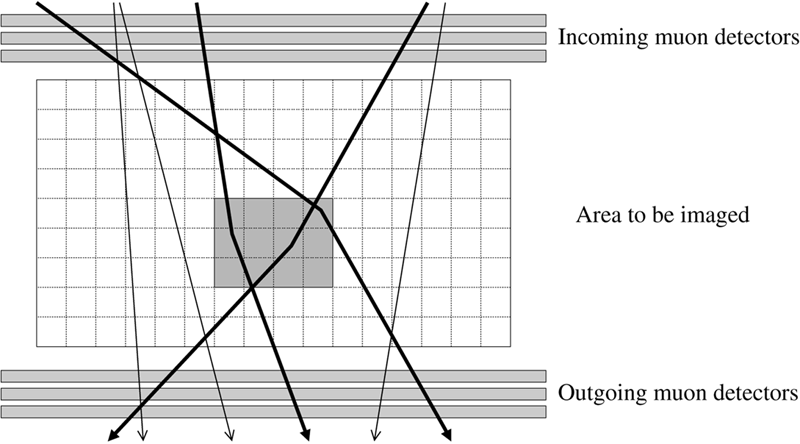
\includegraphics[width=0.8\linewidth]{Chapter5/Figs/Raster/twoSidedCosmicMuon_schults2007.png}
 \captionof{figure}{An side on view of two sided cosmic $\mu$ tomography the detectors are of similar size or larger than the object that is being measured in order to make coincided measurements using cosmic $\mu$ seen in the scattered (black) cosmic $\mu$ from \cite{schultz_2007}.}
 \label{fig:twoSidedCosmicMuonTomographySchults}
\end{figure}
 
 One sided cosmic $\mu$ tomography is when one detector is used to measure the cosmic $\mu$ incidence an example of which can be seen in figure \ref{fig:TopDownCircularWallPlot}. Figure \ref{fig:TopDownCircularWallPlot} is an extremely simplified case where there is a singular wall which blocks 50\,\% of cosmic $\mu$ incidence. However, such a scenario is unlikely except for extremely high Z materials \cite{schultz_2007}. A more realistic example would be in figure \ref{fig:TopDownCircularCubePlot} where the increasing amount of material corresponds with a decreasing attenuation producing a curve shape in the occluded angles of $\phi$. The top down perspective in figures \ref{fig:TopDownCircularWallPlot} \ref{fig:TopDownCircularCubePlot} only show the azimuthal angle ($\phi$). In spherical polar coordinates there is also a polar angle commonly denoted as $\theta$. Figure \ref{fig:sphericalPolarCoordinateSystem} represents both angles in the spherical polar coordinate system. If figure \ref{fig:TopDownCircularCubePlot} is taken and analysed in both $\theta$ and $\phi$ a 360$^\circ$ panoramic view is produced in figure \ref{fig:thetaVsPhiExpectedCube}.
 
 \begin{figure}[htbp]
 \centering
 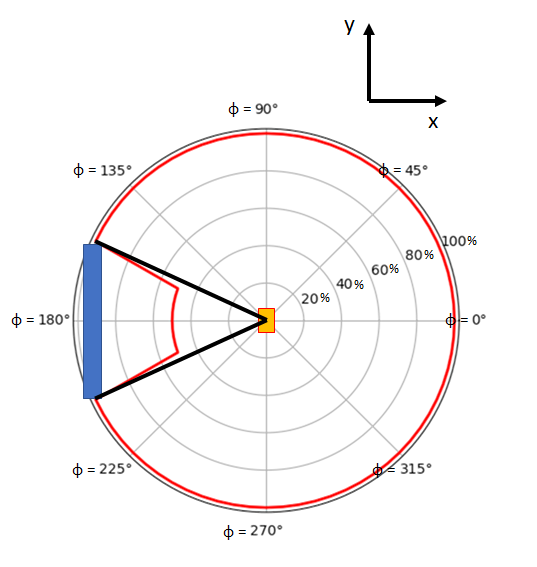
\includegraphics[width=0.5\linewidth]{Chapter5/Figs/wylfaRasterNew/TopDownCircularWallPlot.png}
 \captionof{figure}{How a thin dense wall that blocks 50\,\% of cosmic $\mu$ incidence would look from a top down perspective. A sharp drop in incidence at the edges with no further attenuation. } 
 \label{fig:TopDownCircularWallPlot}
\end{figure}
 
 \begin{figure}[htbp]
 \centering
 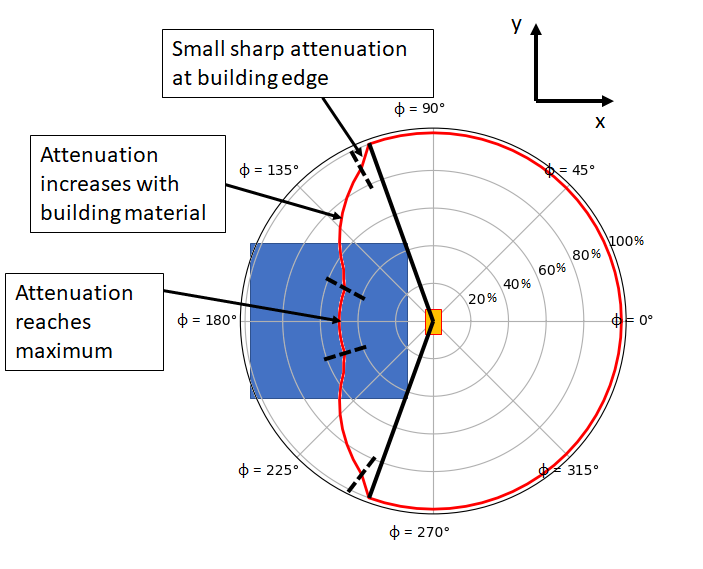
\includegraphics[width=0.7\linewidth]{Chapter5/Figs/wylfaRasterNew/TopDownCircularCubePlot.png}
 \captionof{figure}{How a cube of material would block cosmic $\mu$ incidence from a top down perspective. The amount of attenuation corresponds to the amount of material in the path of the cosmic $\mu$.} 
 \label{fig:TopDownCircularCubePlot}
\end{figure}

 \begin{figure}[htbp]
 \centering
 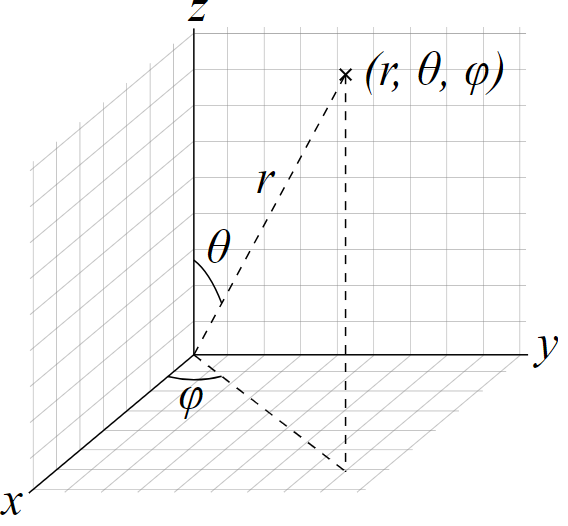
\includegraphics[width=0.5\linewidth]{Chapter5/Figs/wylfaRasterNew/sphericalPolarCoordinatesystem.png}
 \captionof{figure}{The spherical polar coordinate system typically used in physics with the azimuthal angle denoted by $\phi$ and the polar angle denoted by $\theta$. Taken from Wikipedia (\url{https://en.wikipedia.org/wiki/Spherical_coordinate_system}).} 
 \label{fig:sphericalPolarCoordinateSystem}
\end{figure}

 \begin{figure}[htbp]
 \centering
 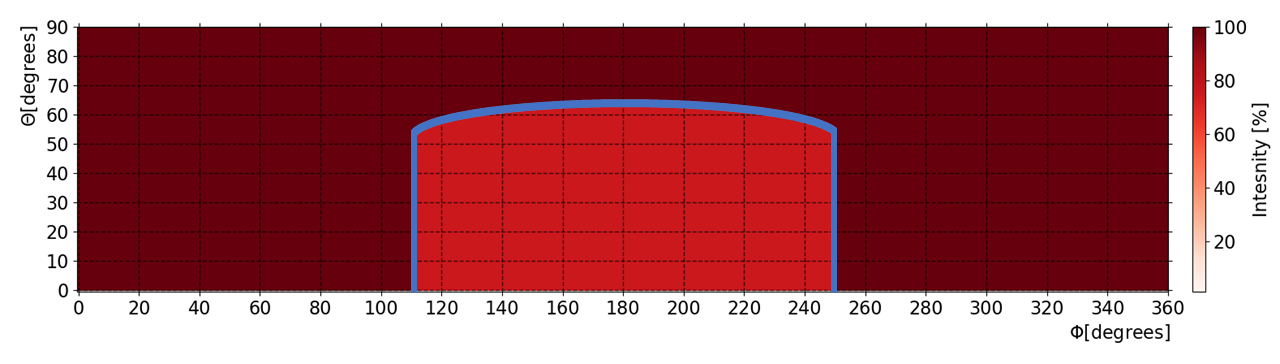
\includegraphics[width=\linewidth]{Chapter5/Figs/wylfaRasterNew/thetaVsPhiExpectedCube.png}
 \captionof{figure}{How the example seen in figure \ref{fig:TopDownCircularCubePlot} can be represented in $\theta$ and $\phi$. Assuming a it's a cuboid.} 
 \label{fig:thetaVsPhiExpectedCube}
\end{figure}

For figure \ref{fig:thetaVsPhiExpectedCube} there is a slight distortion caused at the top of the building due to the projection of a hemispherical distribution onto a cuboid detector. The amount of distortion will also vary depending on the distance from the detector and the size and shape of the building in question. For example a longer shorter building would have significantly more distortion than a tall narrow building. Also the slope of the distortion will vary depending on the position relative to the detector. Further in figure \ref{fig:thetaVsPhiExpectedCube} the drop in intensity is would not be expected to be instantaneous, there would be a gradual decrease in intensity resulting in blurred edges around the occlusion pattern or ``shadow.'' These effects will vary depending on the setup. The VIDARR prototype and upgraded VIDARR detectors for example are cuboid detectors that analyse the whole hemisphere at once, and as such can be considered as 360$^\circ$ cosmic camera rather than as a cosmic $\mu$ telescope in the strictest sense. 
\\\\This is an important consideration as the other cosmic $\mu$ experiments have a very different experimental setup. For example the DIAPHANE experimental setup seen in figure \ref{fig:DIAPHANE_deployment} shows a cosmic $\mu$ telescope with several different planes clearly analysing a very narrow filed of view this helps significantly in preventing distortions and helps prevent bin migration. This is also the case for the MU-RAY collaboration as seen in figure \ref{fig:muRayDetectors} with a tear down of the interorir of a pannel vsiible in figure \ref{fig:muRaySetup}. Both of these are traditional cosmic $\mu$ telescopes as opposed to VIDARR which is an $\Bar{\nu_e}$ detector first and a cosmic $\mu$ camera second. Despite this DIAPHANE MU-RAY and VIDARR all use similar technology using plastic scintillating bars and WLS fibres \cite{Carroll_2018} \cite{Marteau_2017} \cite{ANASTASIO2013423}. With DIAPHANE using ``multianode PMT’s''  \cite{Marteau_2017} and VIDARR and MU-RAY using SiPms \cite{Carroll_2018} \cite{ANASTASIO2013423} to read out the information from the WLS fibres. 
\\\\Both DIAPHANE and MU-RAY have taken tomographic data to image their surroundings. With DIAPHANE imaging LA Soufriere of Guadeloupe using cosmic $\mu$ radiography as seen in figure \ref{fig:diaphaneStructualImaging} which shows different density areas of rock which is relevant for volcanology \cite{Marteau_2017}. MU-RAY has also produced results in figure \ref{fig:mtVesuviusMuRayImaging} the thickness of rock expressed in m can be seen \cite{Ambrosino_2014}. Of more interest is figure \ref{fig:mtVesuviusMuRayTransmission} which shows the ``Transmission'' method. The transmission method used in figure \ref{fig:mtVesuviusMuRayTransmission} is obtained by pointing the MU-RAY detector at the sky for a calibration period of one week then pointing the MU-RAY detector at Mt Vesuvius for one week and then taking the ratio of the two data sets \cite{Ambrosino_2014}. This approach of measuring the free sky and the blocked sky and taking the ratio of the two creates an extremely clear image because it takes the background into account. This creates a clear difference in intensity where a transmission 1 represents free sky and a transmission of 0 represents completely blocked sky. This approach is the one that will be used when analysing the Wylfa reactor site due to the effective reduction of background noise effects and the sharpness of the image it provides. 

\begin{figure}[htbp]
 \centering
 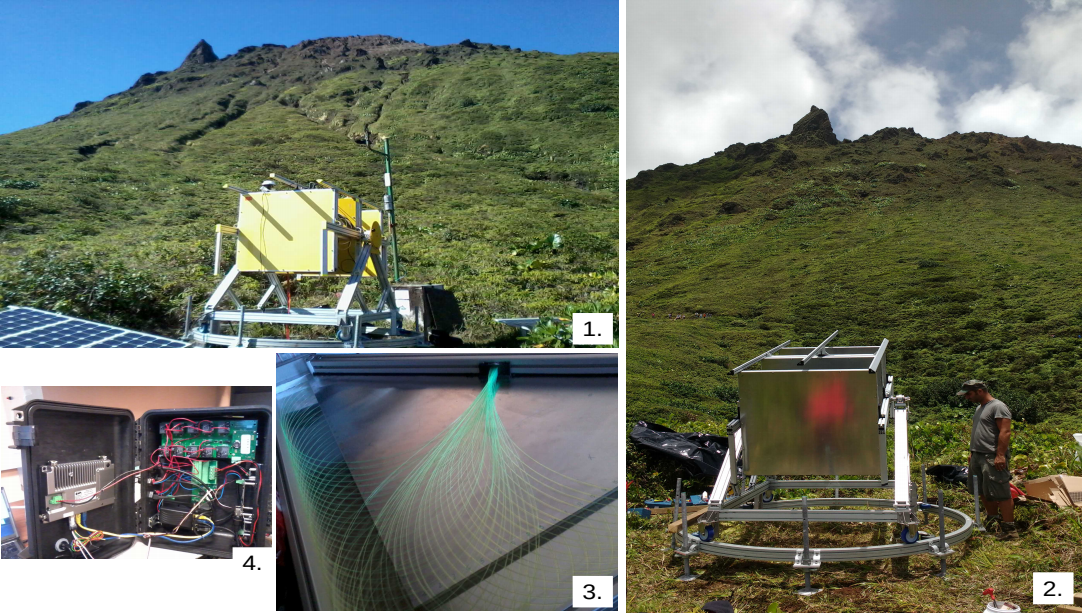
\includegraphics[width=1.0\linewidth]{Chapter5/Figs/Raster/DIAPHANE_deployment.png}
 \captionof{figure}{The deployment of the DIAPHANE detector from \cite{Marteau_2017}. DIAPHANE muon detectors upgrades. 1: the first generation 3 planes muon detector on the slope of La Soufrière of Guadeloupe (PK site). 2: the second generation 3 planes muon detector, with a transverse segmentation divided by a factor 2, on the slope of La Soufrière of Guadeloupe (SAM site). 3: inner WLS fibres collected on a PMT cookie. 4: compact CTRL BOX with embedded hardened processing unit and electronics: common clock signal, WebRelay, Ethernet switch, Power-over-Ethernet to the wifi antenna.} 
 \label{fig:DIAPHANE_deployment}
\end{figure}

\begin{figure}[htbp]
 \centering
 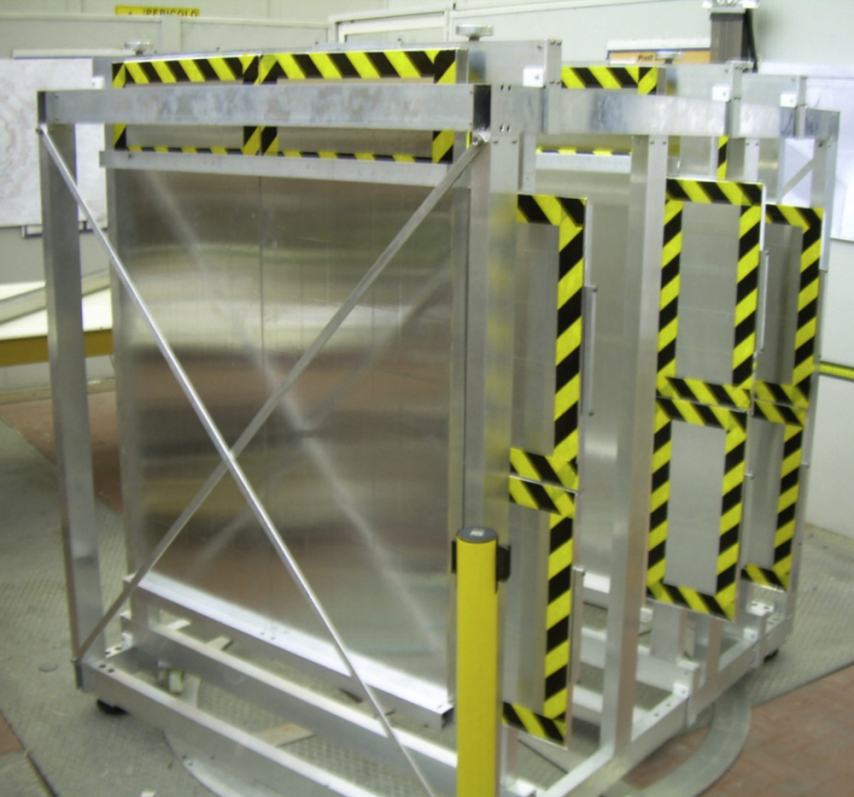
\includegraphics[width=0.7\linewidth]{Chapter5/Figs/Raster/muRayDetectors.png}
 \captionof{figure}{The MU-RAY detector frame with the three X–Y planes mounted. The frame can be oriented using the rotating platform visible at the bottom from \cite{ANASTASIO2013423}} 
 \label{fig:muRayDetectors}
\end{figure}

\begin{figure}[htbp]
 \centering
 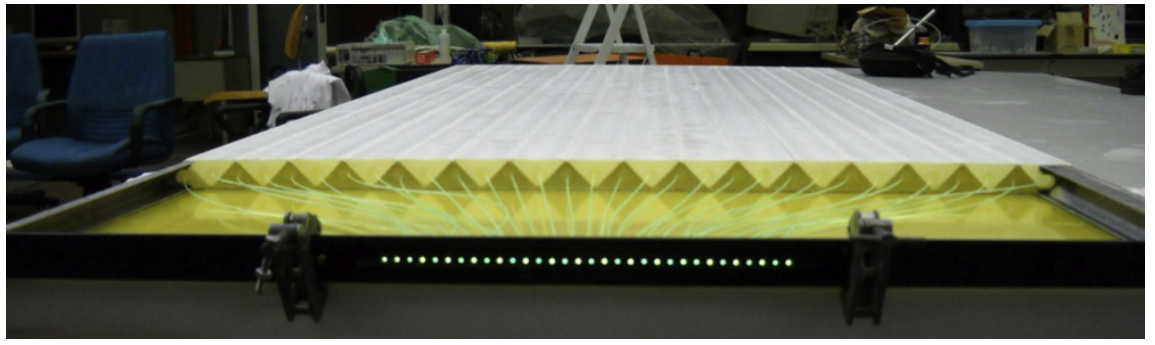
\includegraphics[width=0.7\linewidth]{Chapter5/Figs/Raster/muRaySetup.png}
 \captionof{figure}{The scintillator for the MU-RAY collaboration unlike VIDARR they use triangular prism shaped scintillator \cite{ANASTASIO2013423}.} 
 \label{fig:muRaySetup}
\end{figure}

\begin{figure}[htbp]
 \centering
 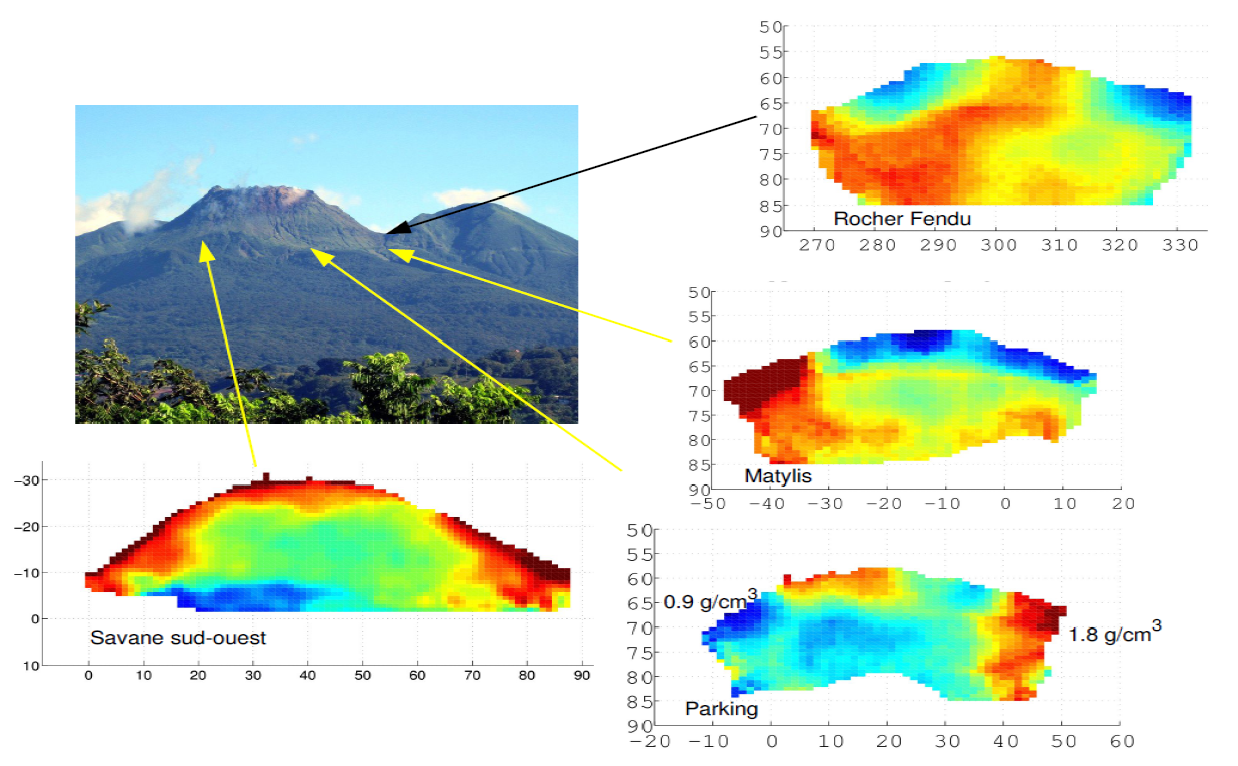
\includegraphics[width=1.0\linewidth]{Chapter5/Figs/Raster/diaphane_structuralImaging.png}
 \captionof{figure}{DIAPHANE structural imaging of the La Soufriere of Guadeloupe dome from 4 different acquisition sites around the dome. The blue areas are the less dense zones of the volcano. The red areas have the highest density. Average density extracted from all those images ranges from 1.6 to 1.8 g.cm$^{-3}$ from \cite{Marteau_2017}} 
 \label{fig:diaphaneStructualImaging}
\end{figure}

\begin{figure}[htbp]
 \centering
 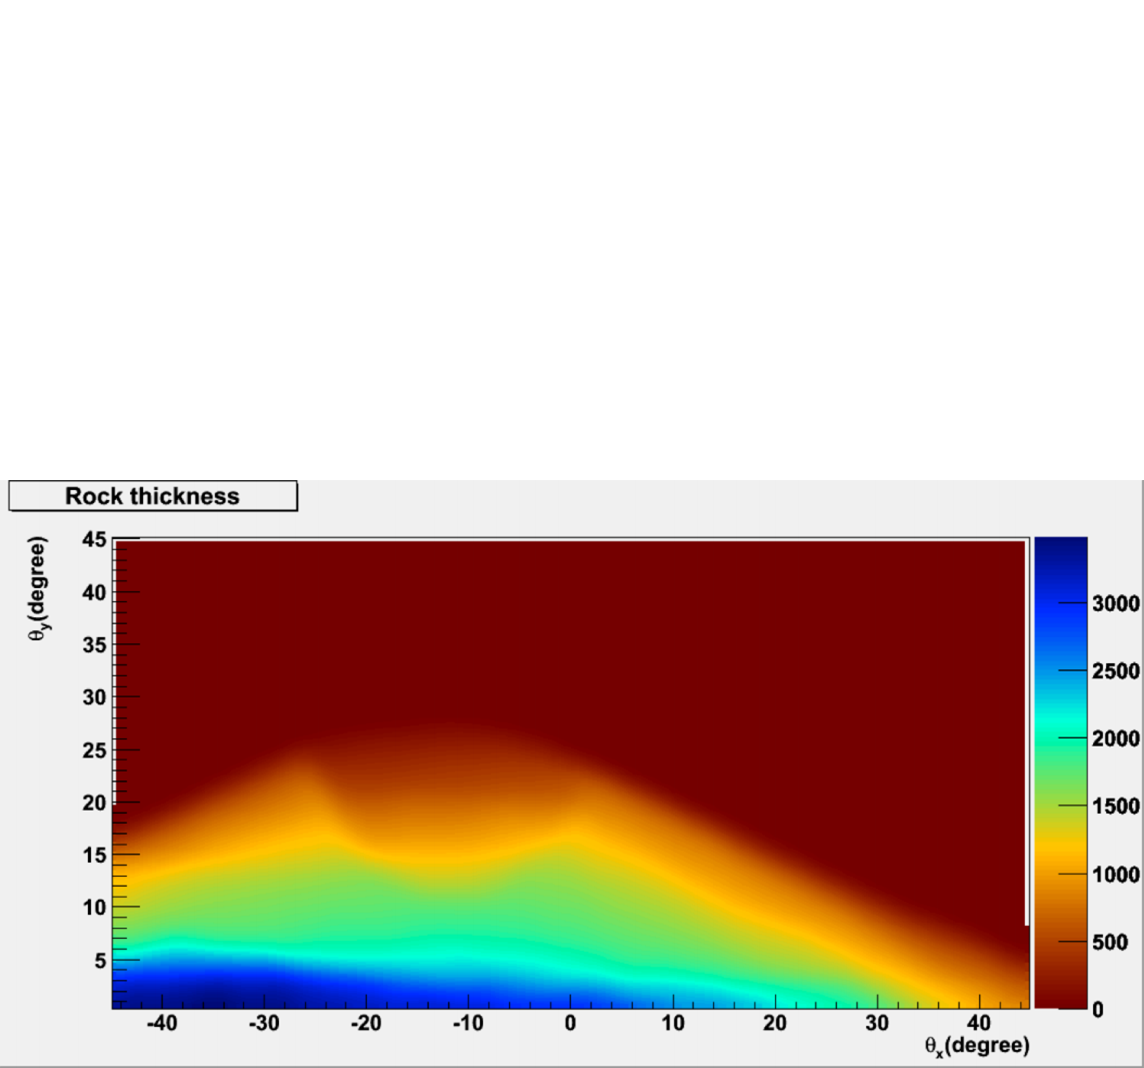
\includegraphics[width=0.7\linewidth]{Chapter5/Figs/Raster/mtVesuviusMuRayImaging.png}
 \captionof{figure}{MU-RAY telescope analysing Vesuvius rock thickness, expressed in m, as seen from the observation point at $\sim$ 800 m altitude. From \cite{Ambrosino_2014}.} 
 \label{fig:mtVesuviusMuRayImaging}
\end{figure}

\begin{figure}[htbp]
 \centering
 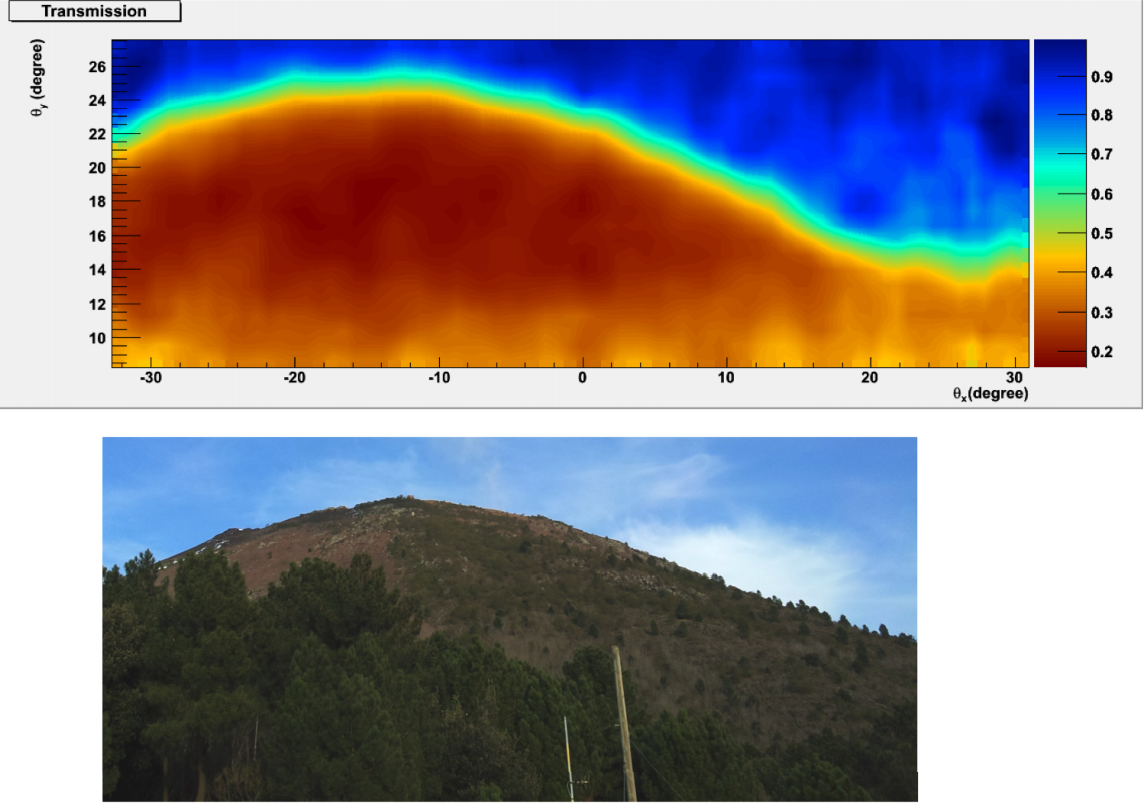
\includegraphics[width=1.0\linewidth]{Chapter5/Figs/Raster/mtVesuviusMuRayTransmission.png}
 \captionof{figure}{MU-RAY data from Vesuvius. Top: the transmission histogram of Mt Vesuvius after one week of data taking. Bottom: a picture of Mt Vesuvius taken by the telescope observation point. From  \cite{Ambrosino_2014}.} 
 \label{fig:mtVesuviusMuRayTransmission}
\end{figure}

\section{Muon Analysis Chain}\label{sec:muonAnalysisChain}
The $\mu$ analysis chain is shown in figure \ref{fig:analysisChain} for calibration of the old detector data an older version of the analysis chain is used based on T2K collaboration analysis chain. For data from the prototype data is extracted from a .mid.gz file then calibrated before being converted into a .root file. The prototypes detector analysed data in cycles of 1.5\,$\mu$s. There are 23 cycles in the prototype detector data from 0 -- 22 with cycle 18 as the trigger cycle and cycles 17 and 19 considered to be underflow and overflow for the trigger signal. The cycles are then interpreted depending on weather the user wants to analyse cosmic $\mu$ data or IBD data. Each cycle will be considered as its own event for cosmic $\mu$ data and the trigger cycles 17 -- 19 are ignored. Whereas the data is split between prompt (cycles 0 -- 16) and delayed (cycles 17 -- 19) for IBD analysis with excess data (cycles 20 -- 22) being ignored. Which mode is decided by convert old detector data so the other programs can interpret the prototype detector data correctly. Simulated data requires minimal changes as it puts data into delayed, prompt and ambiguous categories automatically using truth information. Unfortunately due to the COVID-19 pandemic the calibration and conversion of the new detector data was unable to be constructed as no data exists due to the detector not being constructed. 
 
\begin{figure}[htbp]
 \centering
 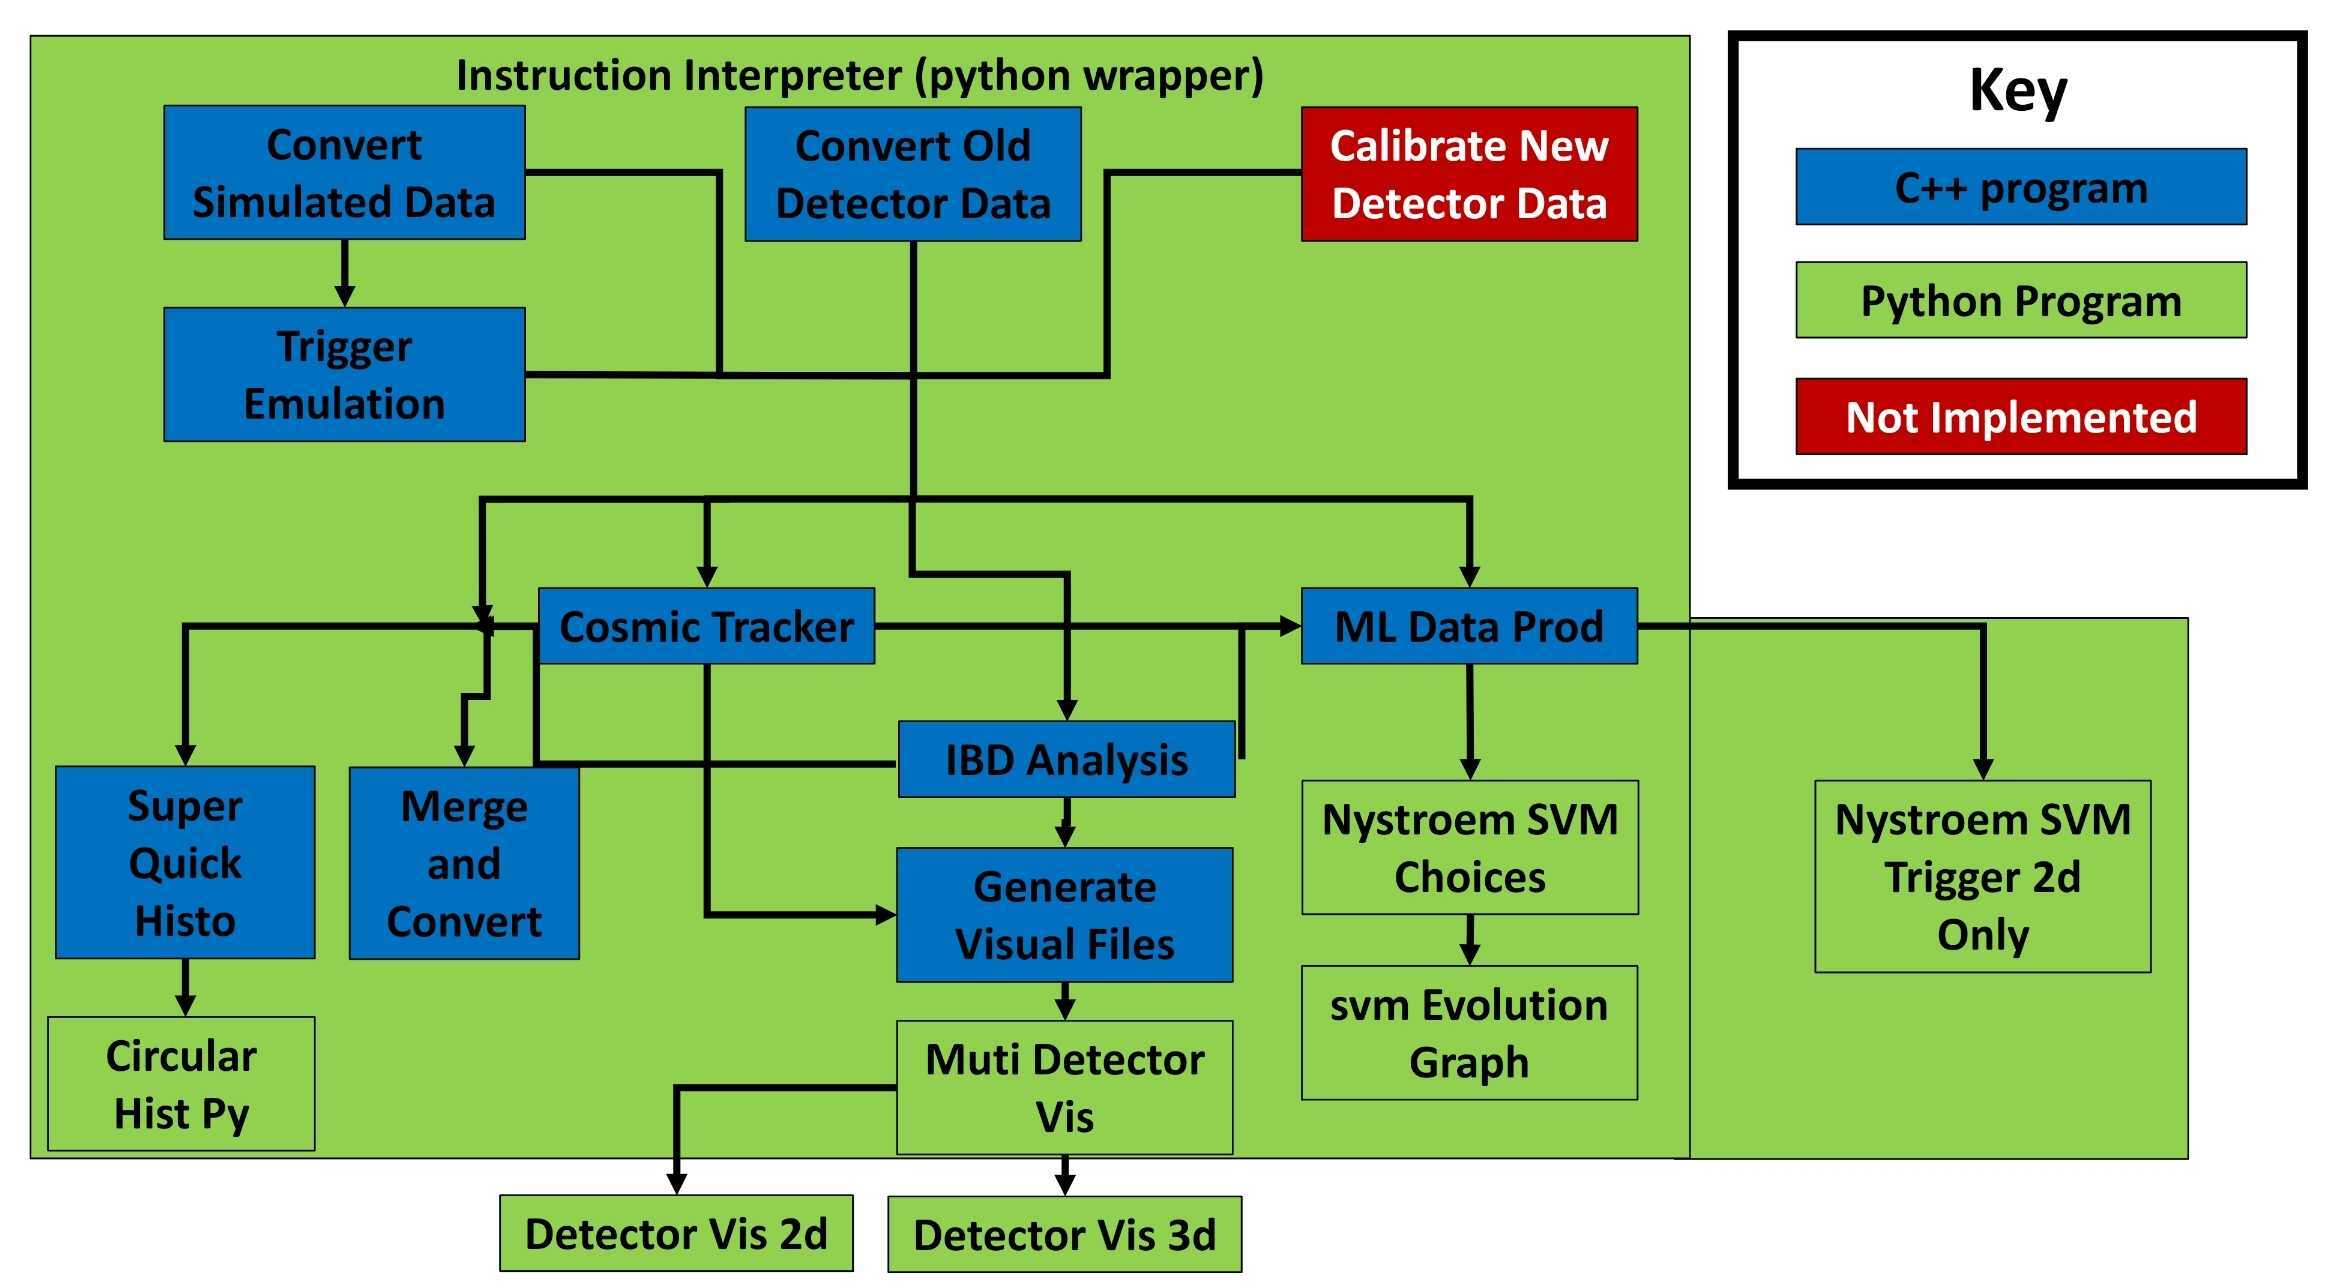
\includegraphics[width=1.0\linewidth]{Chapter5/Figs/Raster/analysisChain.jpg}
 \captionof{figure}{The analysis chain for the detector. It is able to process both simulated and measured data. It uses a combination python programs to handle visualisation and machine learning and c++ programs to process the data. There's a python program that functions as wrapper the instruction interpreter which allows for the creation of macro files to allow for results to be highly replicable. The c++ programs are multithreaded.} 
 \label{fig:analysisChain}
\end{figure}

The cosmic $\mu$ events at Wylfa were taken in accidental coincidence as a result much noise made it into the cosmic $\mu$ data sets. In the raw unprocessed data sets for every 3 cosmic $\mu$ events there are $\sim$ 10000 noise events. As such the SVM machine learning technique previously described in section \ref{sec:MachineLearningTrigger} was used again to filter out the noise. It found the best separating hyper-plane at 8 bars for a threshold of 17.325\,PE (0.693\,MeV) shown in figure \ref{fig:cosmic8BarSignalNoiseCutSVM}. A zoomed in version is also shown in figure \ref{fig:Cosmic8BarSignalNoiseZoomCutSVM} to give a clearer view of the separating line. As seen in figure \ref{subFig:Cosmic8BarNoiseZoomCutSVM} most of the noise is highly concentrated at a low number of bar hits. As a result this is a very effective method of removing the noise. This removes 99.9\,\% of noise and keeps 99\,\% of the cosmic $\mu$ signal so now every 3 cosmic events there are $\sim$ 10 noise events. This greatly improves the signal to noise ratio whilst keeping almost all of the signal. Finding simple effective selection criteria is a task the SVM is well suited to. 

\begin{figure}[htbp]
\centering
\begin{subfigure}{.5\textwidth}
  \centering
  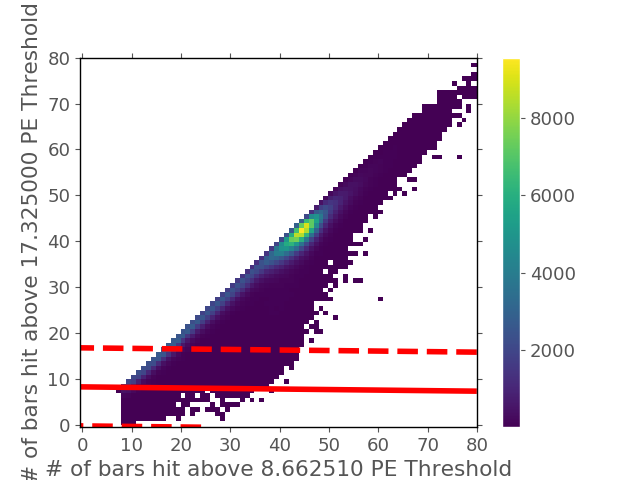
\includegraphics[width=\linewidth]{Chapter5/Figs/Raster/Cosmic8BarSignalCutSVM.png}
  \captionsetup{width=.9\linewidth}
  \caption{8 bar selection criteria for cosmic $\mu$ on measured cosmic data.}
  \label{subFig:cosmic8BarSignalCutSVM}
\end{subfigure}%
\begin{subfigure}{.5\textwidth}
  \centering
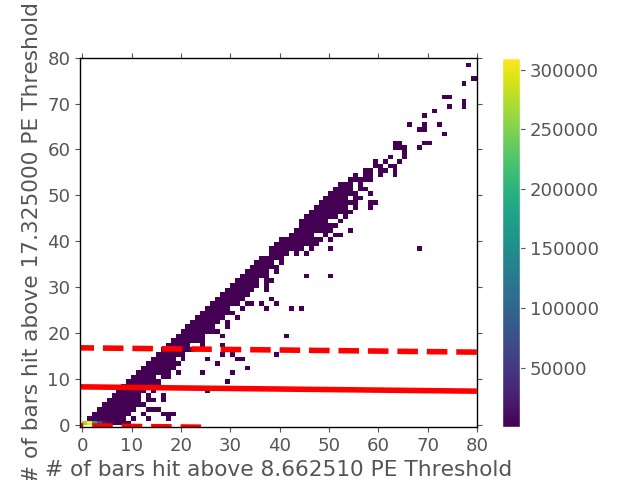
\includegraphics[width=\linewidth]{Chapter5/Figs/Raster/Cosmic8BarNoiseCutSVM.png}
  \captionsetup{width=.9\linewidth}
  \caption{8 bar selection criteria for cosmic $\mu$ on measured noise data.}
  \label{subFig:cosmic8BarNoiseCutSVM}
\end{subfigure}
\caption{How an SVM classifier separates out measured cosmic $\mu$ data it settled on an 8 bar cut above 17.325\,PE (0.693\,MeV). Where everything above the solid line is considered a cosmic $\mu$ and everything below is considered noise.The logic for the SVM classifier is outlined in figure \ref{sec:MachineLearningTrigger}.}
\label{fig:cosmic8BarSignalNoiseCutSVM}
\end{figure}

\begin{figure}[htbp]
\centering
\begin{subfigure}{.5\textwidth}
  \centering
  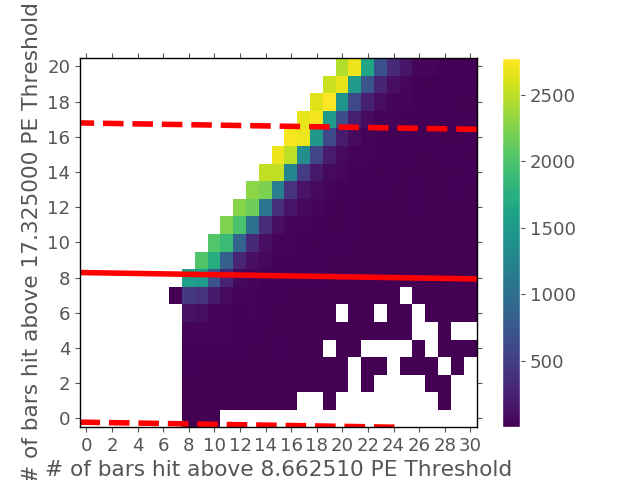
\includegraphics[width=\linewidth]{Chapter5/Figs/Raster/Cosmic8BarSignalZoomCutSVM.png}
  \captionsetup{width=.9\linewidth}
  \caption{Figure \ref{subFig:cosmic8BarSignalCutSVM} zoomed in to show how few cosmic events are removed.} 
  \label{subFig:cosmic8BarSignalZoomCutSVM}
\end{subfigure}%
\begin{subfigure}{.5\textwidth}
  \centering
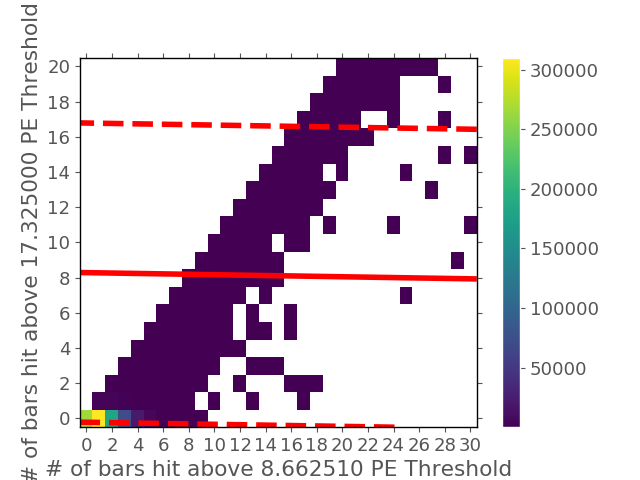
\includegraphics[width=\linewidth]{Chapter5/Figs/Raster/Cosmic8BarNoiseZoomCutSVM.png}
  \captionsetup{width=.9\linewidth}
  \caption{Figure \ref{subFig:cosmic8BarNoiseCutSVM} zoomed in to show how many noise events are clustered around small bar hits.}
  \label{subFig:Cosmic8BarNoiseZoomCutSVM}
\end{subfigure}
\caption{Zoomed in version of figure \ref{fig:cosmic8BarSignalNoiseCutSVM} to show how effective the SVM is at removing noise.}
\label{fig:Cosmic8BarSignalNoiseZoomCutSVM}
\end{figure}

Finally when analysing the response for cosmic $\mu$ event some cycles are correlated to the trigger cycle 18. These cycles are considered as ``bad'' for cosmic $\mu$ data because they are biased towards the trigger cycles these bad cycles are shown in figure \ref{fig:badCycles}. Weather a cycle is considered bad depends on weather or not its count rate is above count rate for cycle 20 in figure \ref{fig:badCycles}. If these bad cycles are added into the data set strange biasing occurs at the side left hand side of side A and side B as seen in figure \ref{fig:sideABHitsWithBadCycles}. These results are a direct effect of the electronic biasing when taking cosmic $\mu$ data in accidental coincidence and are not a result of track fitting as shown later in figures \ref{fig:wylfaSideABHits} and \ref{fig:liverpoolSideABHits} the track fitter does not seem to cause any biasing. 

\begin{figure}[htbp]
 \centering
 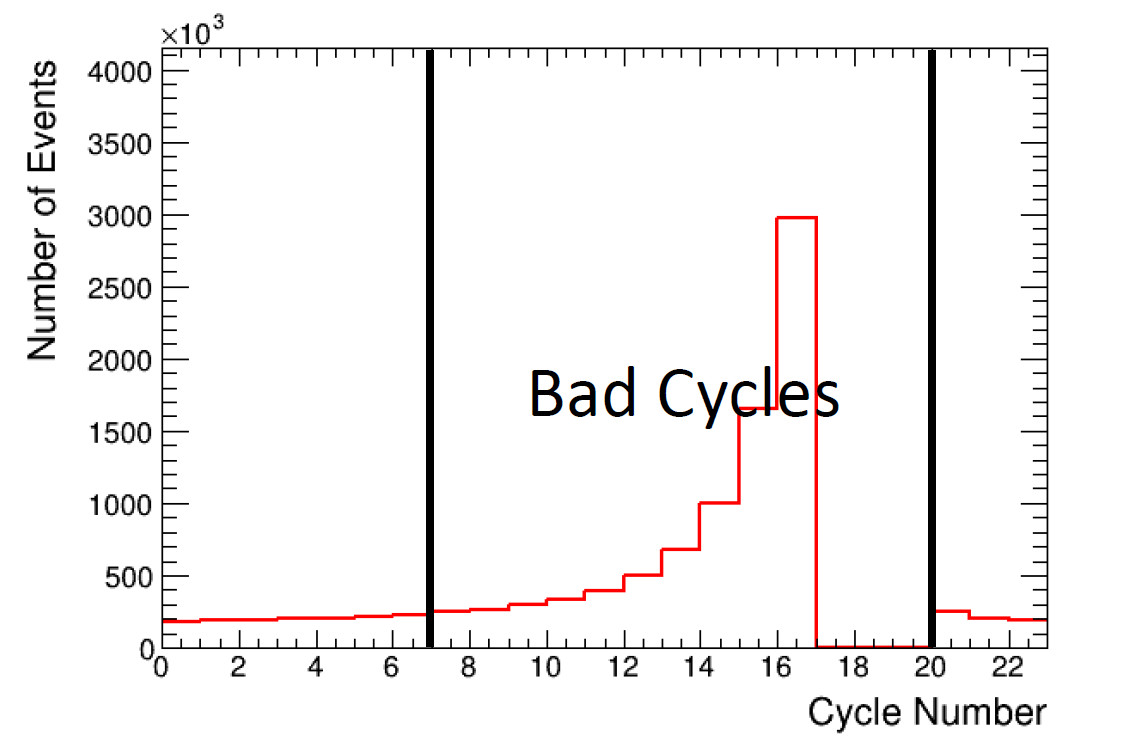
\includegraphics[width=0.7\linewidth]{Chapter5/Figs/Raster/badCycles.png}
 \captionof{figure}{The bad cycles (trigger cycles 17,18 and 19 already removed) for cosmic $\mu$ in the measured data for the Wylfa data set. Weather a cycle is considered ``bad'' depends on how much the cycle correlates to the trigger cycles.} 
 \label{fig:badCycles}
\end{figure}

\begin{figure}[htbp]
\centering
\begin{subfigure}{.5\textwidth}
  \centering
  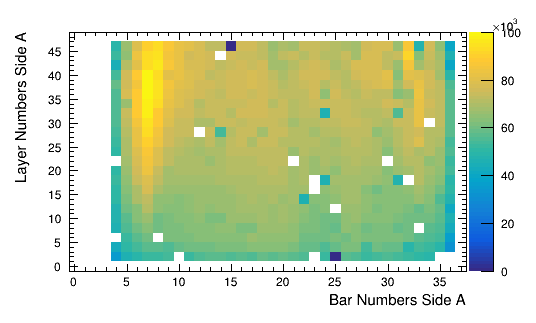
\includegraphics[width=\linewidth]{Chapter5/Figs/Raster/sideAHitsWithBadCycles.png}
  \captionsetup{width=.9\linewidth}
  \caption{Side A cosmic $\mu$ hits reconstructed with bad cycles included.} 
  \label{subFig:sideAHitsWithBadCycles}
\end{subfigure}%
\begin{subfigure}{.5\textwidth}
  \centering
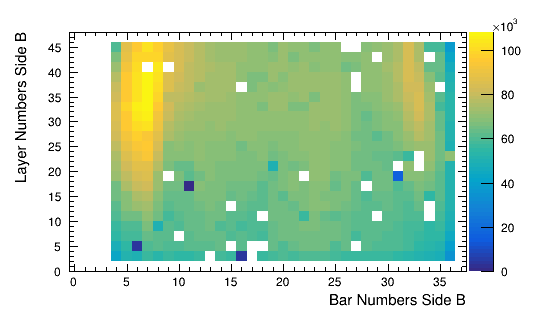
\includegraphics[width=\linewidth]{Chapter5/Figs/Raster/sideBHitsWithBadCycles.png}
  \captionsetup{width=.9\linewidth}
  \caption{Side B cosmic $\mu$ hits reconstructed with bad cycles included.}
  \label{subFig:sideBHitsWithBadCycles}
\end{subfigure}
\caption{The detector hits for cosmic $\mu$ when reconstructed with a tracker when bad cycles are included. Large streaks are visible on the left hand sides of both side A and side B.}
\label{fig:sideABHitsWithBadCycles}
\end{figure}

\section{Deployment At Wylfa}\label{sec:deploymentAtWylfa}
The original prototype detector was deployed at the Wylfa Nuclear power station from 07-07-2014 to 25-02-2016 with data being taken continuously over that time period both with the reactor on and off with inverse $\beta$ decay measurements seen in figure \ref{fig:prototypeMeasumentFlux}. The placement of the detector in relation to the Wylfa reactor buildings can be seen in figure \ref{fig:DetectorPositionTopDown} the reactors were placed either end of the main reactor building in the centre of the cylindrical shaped ends at either end of the ``dog bone.'' Whilst there is no good height data for the buildings at the Wylfa reactor site there is a drone picture available seen in figure \ref{fig:wylfaAir}. In figure \ref{fig:wylfaAir} the tallest buildings are clearly visible, of particular importance is the main reactor building and the turbine hall. The service buildings in between the turbine hall and the  main reactor building are also very important as they are much closer to the detector's position as seen in figure \ref{fig:DetectorPositionTopDown} and so will appear taller than the main reactor building. Also in figures \ref{fig:DetectorPositionTopDown} \ref{fig:wylfaAir} the steam bridges that connect the main reactor building and the turbine hall are also visible. The steam bridges are not large buildings and are approximated to be 5\,m thick and 10\,m off of the ground in simulation. But one of the steam bridges is very close to the detector as can be seen in figure \ref{fig:DetectorPositionTopDown} and so will occlude a significant portion of the $\phi$ $\theta$ space the detector observes. 

\begin{figure}[htbp]
 \centering
 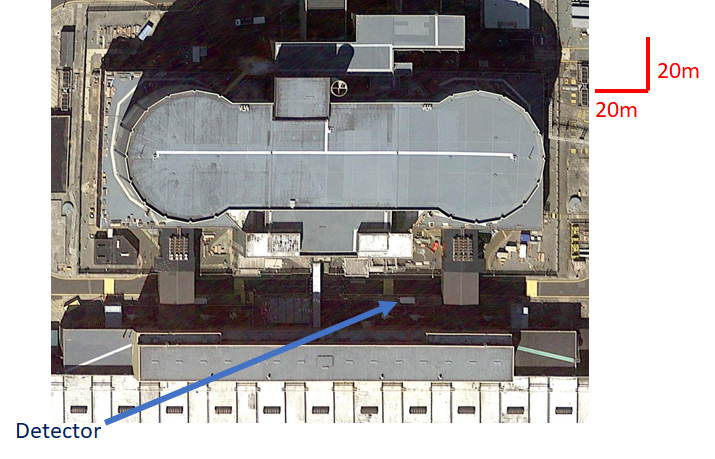
\includegraphics[width=0.75\linewidth]{Chapter5/Figs/wylfaRasterNew/DetectorPositionTopDown.png}
 \captionof{figure}{Google Maps aerial photography image, displaying the power plant site as well as the approximate detector position. The detector is in the middle of many site buildings occluding the incident cosmic rays. Key buildings shown are the reactor building, the turbine hall and the steam pipe connections between the two \cite{GoogleMapsWylfaLink}.} 
 \label{fig:DetectorPositionTopDown}
\end{figure}

\begin{figure}[htbp]
 \centering
 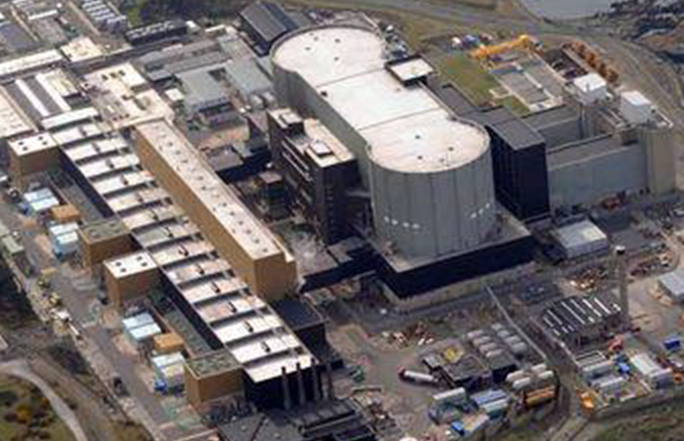
\includegraphics[width=0.6\linewidth]{Chapter5/Figs/Raster/wylfaArielView.png}
 \captionof{figure}{An aerial view of the Wylfa power station the main reactor building is the the shape of a "dog bone" the detector was placed in-between the turbine hall and reactor building. Edited from \cite{wylfaDronePictureLink}.} 
 \label{fig:wylfaAir}
\end{figure}

In addition the structure of the buildings needs to be considered as well. An example of the reactor building structure is seen in figure \ref{fig:wylfaReactorRoughStructure} with the top half of the structure being air wrapped in a concrete skin and the bottom half being thick concrete shielding. As a result any cosmic $\mu$ events that traverse through the top of the section will have a much greater chance to get through than those traversing at lower angles of $\theta$. This will have two important impacts on the data set firstly it will mean that the tops of the buildings will be ``blurred'' to some extent as the amount of material will be initially low. Secondly the it will mean that the transmission value will decrease with the $\theta$ value where the reactor buildings are observed but especially where the reactor core and reactor core shielding will be located. 

\begin{figure}[htbp]
 \centering
 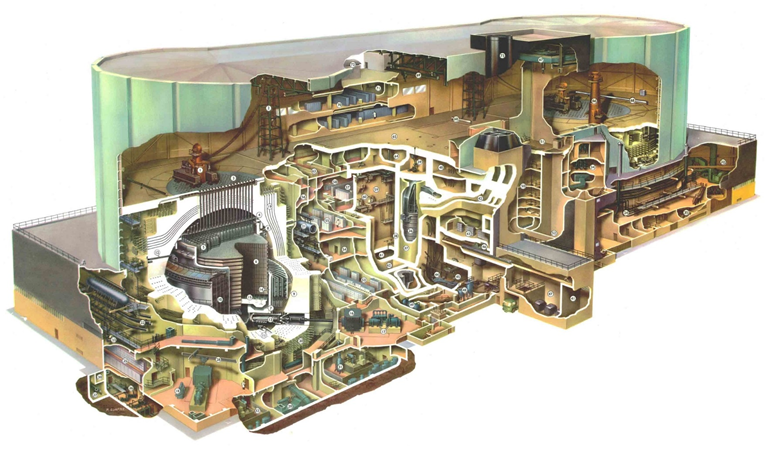
\includegraphics[width=0.6\linewidth]{Chapter5/Figs/wylfaRasterNew/wylfaReactorRoughStructure.png}
 \captionof{figure}{A cut away diagram from \cite{neiMag_1965}. Shows the internal structure of the Wylfa from the back of the reactor buildings the bottom half of the reactor buildings have thick concrete walls whilst the upper section is mostly storage. As this is an qualitative illustration of the building for public communication, the exact details, locations of features and proportions may not match the exact physical structure.} 
 \label{fig:wylfaReactorRoughStructure}
\end{figure}

\section{Simulation of Cosmic Muon Hemisphere}\label{sec:SimulationOfCosmics}
Before the data could be analysed a simulation of cosmic $\mu$ using a cosmic hemisphere was used in order to quantify segmentation effects and any other detector effects. These can be quite significant as seen in figures \ref{fig:phiGenVsRecoHem} and \ref{fig:cirPhiGenVsRecoHem} the reconstruction of our detector can be quite adversely effected by vertical events. If an event is vertical in one side of the detector then the other side will dominate as such it results in spikes at 0$^\circ$, 90$^\circ$, 180$^\circ$, 270$^\circ$. This bin migration is caused by the detector being a segmented cuboid, any segmented cuboid detector as the projection of a smooth hemispherical distribution will not map cleanly onto cuboid. Figures \ref{fig:cosmicBinMigrationSideA} and \ref{fig:cosmicBinMigrationSideB} show how the segmentation of the VIDARR detector causes bin migration. For figure \ref{fig:cosmicBinMigrationSideA} angles of $\phi$ are solely determined by angle in side A the same is true for side B in figure \ref{fig:cosmicBinMigrationSideB}. 

\begin{figure}[htbp]
 \centering
 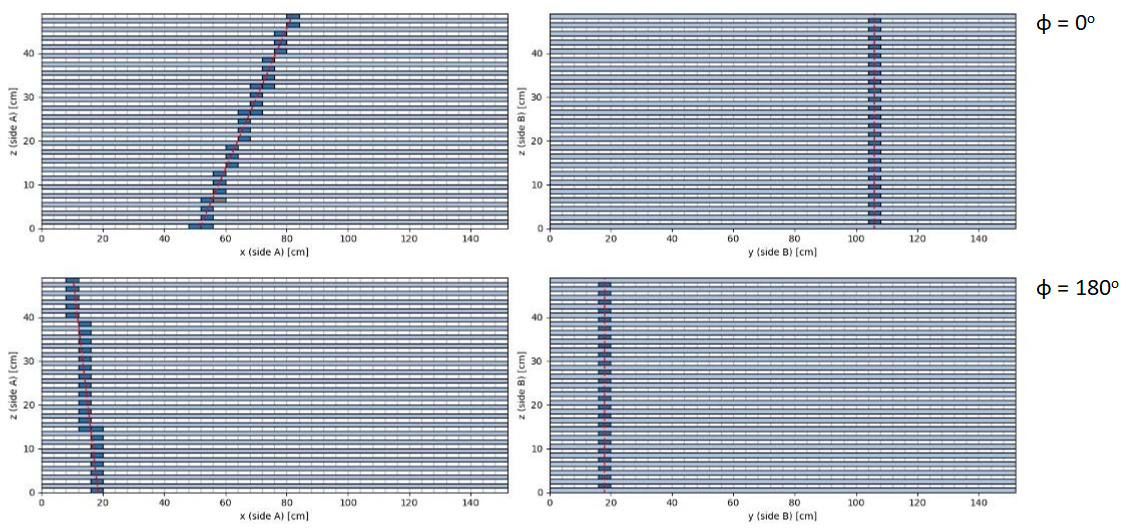
\includegraphics[width=\linewidth]{Chapter5/Figs/cosmicBinMigrationSideA.png}
 \captionof{figure}{Side A Bin migration due to the segmentation size of VIDARR. In this example side B has no $\phi$ component and so any value on side A determines $\phi$ exclusively warping the distribution. \hl{this plot is old and needs to be redone with current colour scheme}.} 
 \label{fig:cosmicBinMigrationSideA}
\end{figure}

\begin{figure}[htbp]
 \centering
 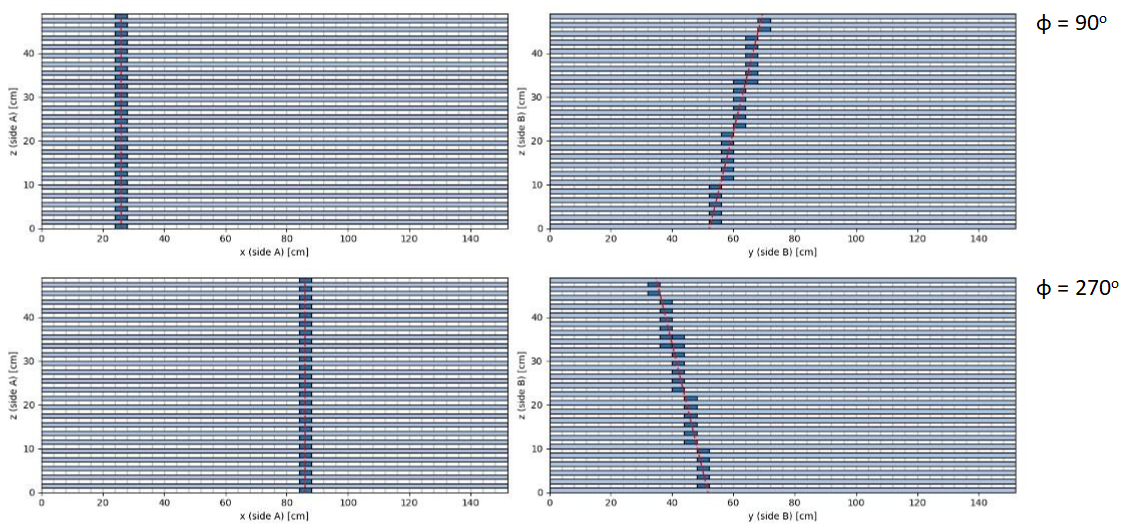
\includegraphics[width=\linewidth]{Chapter5/Figs/cosmicBinMigrationSideB.png}
 \captionof{figure}{Side B Bin migration due to the segmentation size of VIDARR. In this example side A has no $\phi$ component and so any value on side B determines $\phi$ exclusively warping the distribution.\hl{this plot is old and needs to be redone with current colour scheme}.} 
 \label{fig:cosmicBinMigrationSideB}
\end{figure}

However this is only true with $\phi$, bin migration is significantly less pronounced in $\theta$ as seen in figure \ref{fig:thetaGenVsRecoHem}. Significant bin migration is is only seen in bins 0$^\circ$, 5$^\circ$, 80$^\circ$, 85$^\circ$, 90$^\circ$ but bins 10$^\circ$ -- 75$^\circ$ are accurately reconstructed. The large discrepancy in bin migration between $\theta$ and $\phi$ is due to the size of the segments in the VIDARR detector as they are 4\,cm wide by 1\,cm tall they are able to more accurately reconstruct information vertically than in any other direction. Which is useful for reconstructing vertical information such as the height of buildings. Though as will be outlined in section \ref{sec:cosmicTrackerUncertainties} the segmentation and effect of corner clipping events makes reconstruction of $\theta$ more difficult than expected. When comparing the generated hit map in figure \ref{fig:rawHemisphereFiducialBarsSideAB} for a cosmic the $\mu$ hemisphere the reconstruction appears to be very accurate in figure \ref{fig:HemisphereFiducialBarsSideAB}. From this it is reasonable to assume that the tracker not introducing any biases into the generated data set.

\begin{figure}[htbp]
 \centering
 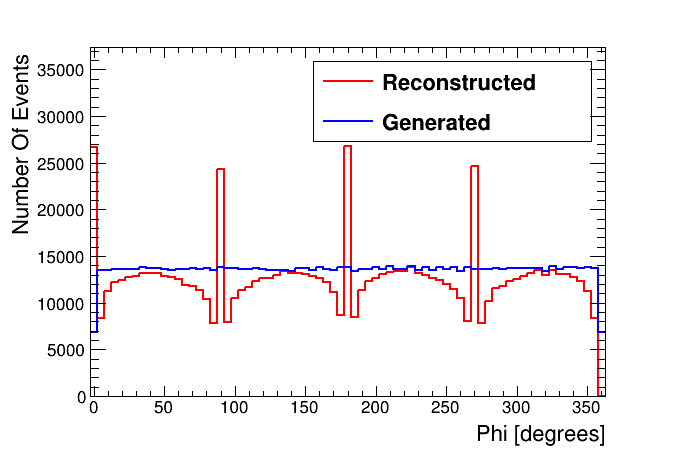
\includegraphics[width=0.8\linewidth]{Chapter5/Figs/Raster/hemispherePhiCompare.png}
 \captionof{figure}{Generated $\phi$ vs reconstructed $\phi$ with the online track fitter for a cosmic hemisphere distribution} 
 \label{fig:phiGenVsRecoHem}
\end{figure}

\begin{figure}[htbp]
 \centering
 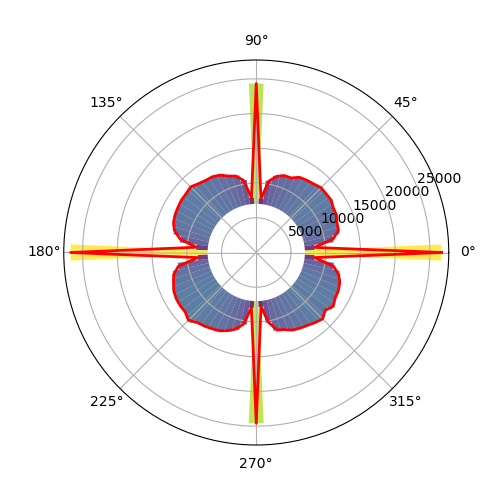
\includegraphics[width=0.6\linewidth]{Chapter5/Figs/Raster/cosmicSimpleHemNoDead_Ciruclarphi.png}
 \captionof{figure}{Circular plot of the reconstructed $\phi$ for a simulated cosmic hemisphere.} 
 \label{fig:cirPhiGenVsRecoHem}
\end{figure}


\begin{figure}[htbp]
 \centering
 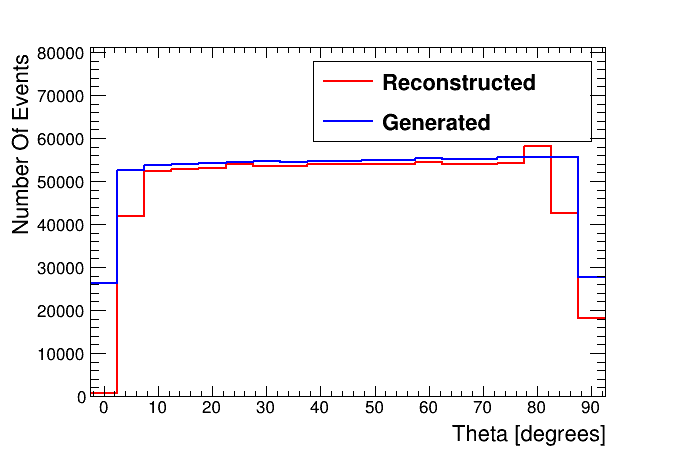
\includegraphics[width=0.8\linewidth]{Chapter5/Figs/Raster/hemisphereThetaCompare.png}
 \captionof{figure}{Generated $\theta$ vs reconstructed $\theta$ for a cosmic hemisphere distribution} 
 \label{fig:thetaGenVsRecoHem}
\end{figure}

\begin{figure}[htbp]
\centering
\begin{subfigure}{.5\textwidth}
  \centering
  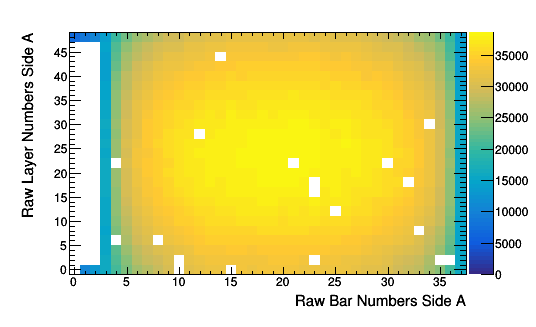
\includegraphics[width=\linewidth]{Chapter5/Figs/Raster/rawHemisphereFiducialBarsSideA.png}
  \captionsetup{width=.9\linewidth}
  \caption{Generated bars hit for side A.}
  \label{subFig:rawHemisphereFiducialBarsSideA}
\end{subfigure}%
\begin{subfigure}{.5\textwidth}
  \centering
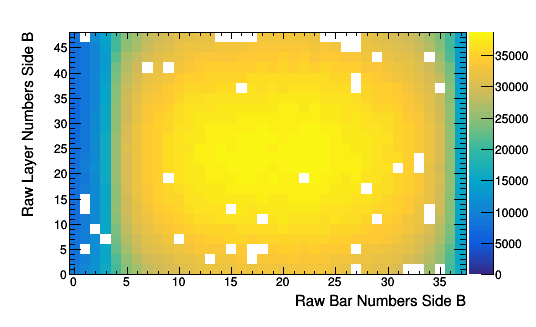
\includegraphics[width=\linewidth]{Chapter5/Figs/Raster/rawHemisphereFiducialBarsSideB.png}
  \captionsetup{width=.9\linewidth}
  \caption{Generated bars hit for side B.}
  \label{subFig:rawHemisphereFiducialBarsSideB}
\end{subfigure}
\caption{Generated hemisphere bars hit when using the generated $\phi$ seen in figure \ref{fig:phiGenVsRecoHem} and generated $\theta$ \ref{fig:thetaGenVsRecoHem}. Dead and un-instrumented channels are simulated to improve accuracy and the simulation bounds match the fiducial bounds.}
\label{fig:rawHemisphereFiducialBarsSideAB}
\end{figure}

\begin{figure}[htbp]
\centering
\begin{subfigure}{.5\textwidth}
  \centering
  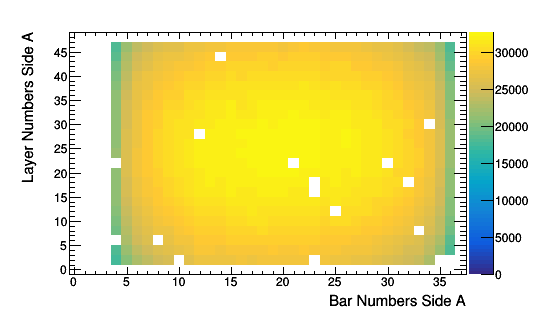
\includegraphics[width=\linewidth]{Chapter5/Figs/Raster/hemisphereFiducialBarsSideA.png}
  \captionsetup{width=.9\linewidth}
  \caption{Reconstructed bars hit for side A.}
  \label{subFig:hemisphereFiducialBarsSideA}
\end{subfigure}%
\begin{subfigure}{.5\textwidth}
  \centering
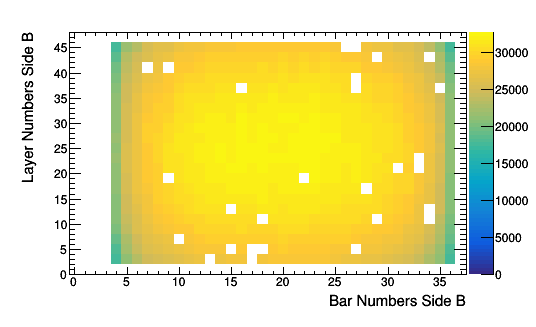
\includegraphics[width=\linewidth]{Chapter5/Figs/Raster/hemisphereFiducialBarsSideB.png}
  \captionsetup{width=.9\linewidth}
  \caption{Reconstructed bars hit for side B.}
  \label{subFig:hemisphereFiducialBarsSideB}
\end{subfigure}
\caption{Reconstructed hemisphere bars hit when using the reconstructed $\phi$ seen in figure \ref{fig:phiGenVsRecoHem} and reconstructed $\theta$ \ref{fig:thetaGenVsRecoHem}. The tracker is not disrupted by the dead channels and accurately reconstructs the hits seen in figure \ref{fig:rawHemisphereFiducialBarsSideAB} with minimal detector corner clipping events removed.}
\label{fig:HemisphereFiducialBarsSideAB}
\end{figure}

In order to quantify the effect of cosmic $\mu$ coming for every possible angle a cosmic hemisphere is simulated. The reconstruction of the cosmic hemisphere done by the tracker can be seen in figure \ref{fig:simulatedHemisphereDist}. The reconstruction artefacts shown in figures \ref{fig:phiGenVsRecoHem} and \ref{fig:thetaGenVsRecoHem} can also be seen to have a dependence on one another in figure \ref{fig:simulatedHemisphereDist}. Apart from the uncertainties introduced from segmentation there are no other uncertainties that are significant that are visible in \ref{fig:simulatedHemisphereDist}. However, this does not mean that that other uncertainties are not present just that the most noticeable uncertainty is due to the segmentation. 
\\\\ When trying to accurately reconstruct all the available cosmic $\mu$ there is no $\chi^2$ selection criteria. This is because many cosmic $\mu$ may shower when inside the detector and as a result may have a high $\chi^2$ but are still an accurate representation of cosmic $\mu$ direction. But a $\chi^2$ cut is effective when trying to accurately measure the $dE/dx$ as seen in figure \ref{fig:dedxGenVsRecoHem} showers produce many secondaries in the detector which when divided by the same length causes an increase in $dE/dx$ which is not justifiable. Therefore for positional reconstruction showers are kept but for online use where calibration is the goal showers are discarded. In this analysis, the reconstruction is optimised for the angle-of-incidence extraction as key analysis variable. The reconstruction steps for fitting each individual track is as follows: 
\begin{enumerate}
  \item \textbf{Energy Threshold:} Exclude all hits below 0.345\,MeV
  \item \textbf{Track Width:} Exclude hits that are 4 bars away from any other hit 
  \item \textbf{Hit Threshold:} Exclude events that have $<$ 4 bars per side that are above a 0.69\,MeV threshold
  \item \textbf{Basic Fit:} Find a basic gradient and intercept using top and bottom hit of the event
  \item \textbf{First Fit:} First fit of the track 
  \item \textbf{Track Width 2:} Exclude hits that are 4.5 bars away from the track
  \item \textbf{Second Fit:} second fit of the track
  \item \textbf{Track Width 3:} Exclude any hits that are 0.5 bars away from the track
  \item \textbf{Third Fit:} Third and final fit of the track
\end{enumerate}
For the following analysis showering events were considered as well to maximise the available data set when taking cosmic $\mu$ in accidental coincidence. For calibration a $\chi^2$ cut would also be implemented. The fitter uses the GNU scientific library simplex minimiser \cite{galassi2002gnu} in order to solve for $y$ = $mx$ + $c$.  

\begin{figure}[htbp]
 \centering
 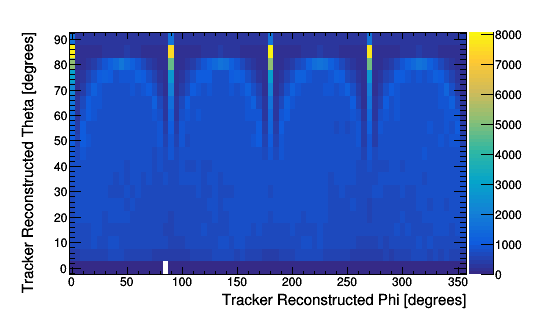
\includegraphics[width=0.8\linewidth]{Chapter5/Figs/Raster/pvsTFiduicalHemisphere.png}
 \captionof{figure}{Simulated cosmic hemisphere which has a flat distribution in $\theta$ from 0$^\circ$ to 90$^\circ$ and a flat distribution in $\phi$ from 0$^\circ$ to 360$^\circ$ which is then reconstructed using the online track fitter} 
 \label{fig:simulatedHemisphereDist}
\end{figure}

\begin{figure}[htbp]
 \centering
 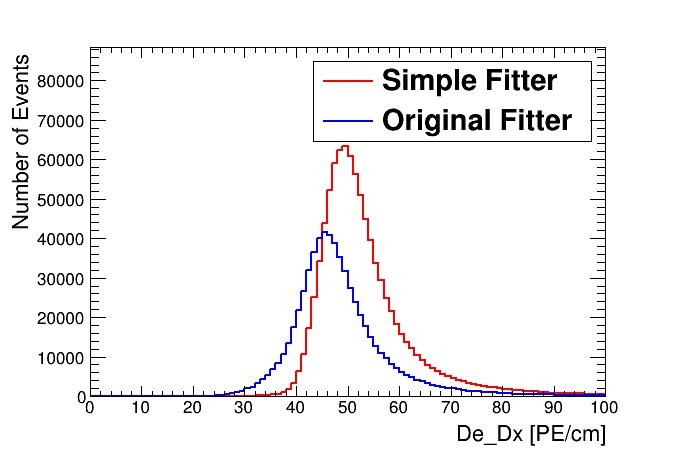
\includegraphics[width=0.8\linewidth]{Chapter5/Figs/Raster/dedxComarison.png}
 \captionof{figure}{\hl{need to add in generated de dx for this ploy} This is also more a show of the $\chi^2$/DOF effects the dE/dx and therefore how that may or may not be useful for online use.} 
 \label{fig:dedxGenVsRecoHem}
\end{figure}

% \begin{figure}[htbp]
%  \centering
%  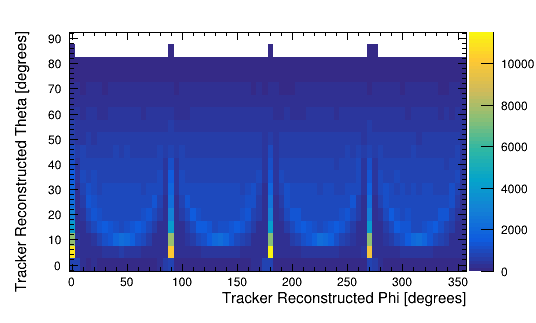
\includegraphics[width=0.8\linewidth]{Chapter5/Figs/Raster/simulatedNormalDistirbution.png}
%  \captionof{figure}{\hl{theta has been reversed now!!!} Simulated distribution with an ideally generated cosmic distribution.} 
%  \label{fig:simulatedNormalDist}
% \end{figure}

\section{Reactor Shadow: Methodology} \label{sec:ReactorShadowMethodology}
When analysing cosmic $\mu$ events it is necessary to have a good understanding of where the buildings that will block cosmic $\mu$ events will be. In figure \ref{fig:DetectorPositionTopDown} the detector position is already known relative to the main reactor buildings that are likely to cast shadows thanks to Google Earth. In figure \ref{fig:wylfaTraceStep1} the buildings have had simple shapes overlaid on top of them with a corresponding key to highlight the buildings of interest. In figure \ref{fig:wylfaTraceStep2} these shapes are then offset to account for the building heights relative to the detector. The most obvious anchor point in figure \ref{fig:wylfaTraceStep2} being the top left of the main reactor building which determines the position of most of the buildings. The turbine hall offset is slightly different. This allows for the angle of the aerial photo and the heights of the buildings to be taken into account. And finally the connecting lines and background aerial photo from figure \ref{fig:wylfaTraceStep2} are removed to produce figure \ref{fig:wylfaTraceStep4} thus producing the final clean trace. In figures \ref{fig:wylfaTraceStep1}  -- \ref{fig:wylfaTraceStep4} the size of the reactor core area is roughly inferred from private communications to be a cylinder with a diameter of $\sim$ 25\,m including both the reactor core and corresponding shielding. This inference is later corroborated with measurements of the Wylfa data. 

\begin{figure}[htbp]
 \centering
 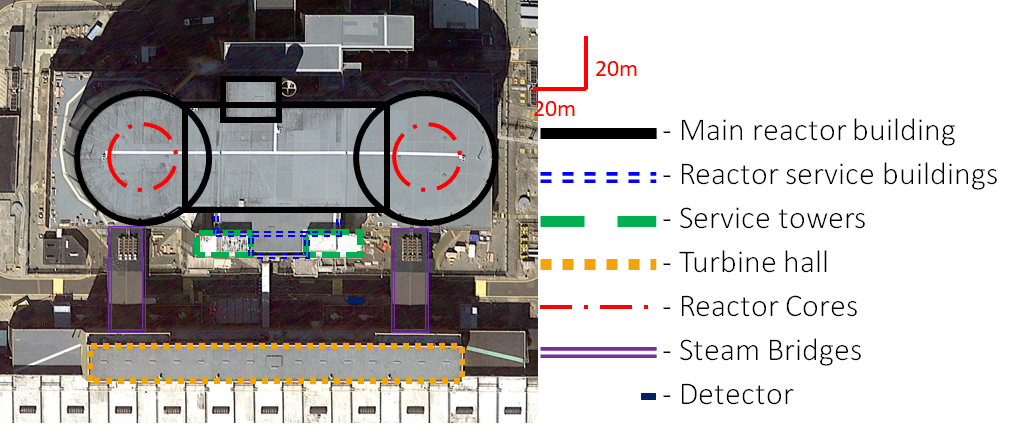
\includegraphics[width=\linewidth]{Chapter5/Figs/wylfaRasterNew/wylfaTraceStep1.png}
 \captionof{figure}{A basic trace on top of figure \ref{fig:wylfaAir}. Basic shapes are overlaid on top of the buildings at Wylfa.} 
 \label{fig:wylfaTraceStep1}
\end{figure}

\begin{figure}[htbp]
 \centering
 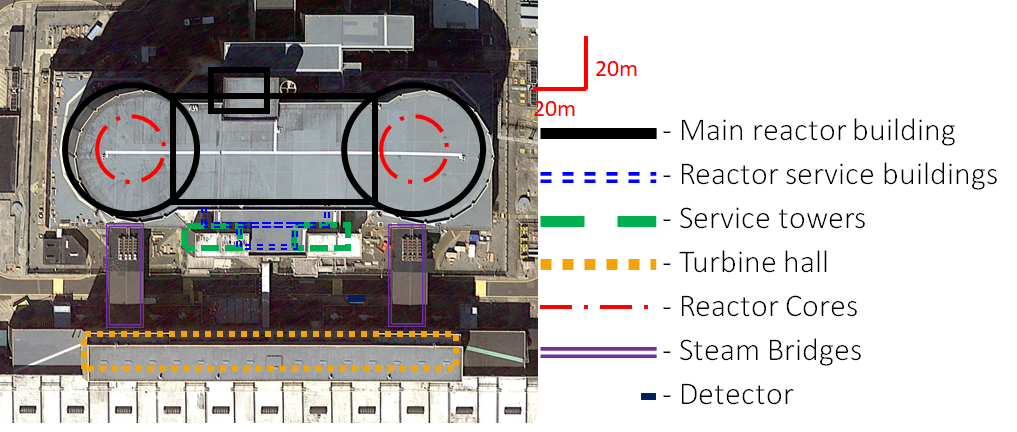
\includegraphics[width=\linewidth]{Chapter5/Figs/wylfaRasterNew/wylfaTraceStep2.png}
 \captionof{figure}{Figure \ref{fig:wylfaTraceStep1} with the trace adjusted to take the satellite position into account. By taking the base of the buildings and moving the trace towards the base of the buildings.} 
 \label{fig:wylfaTraceStep2}
\end{figure}

% \begin{figure}[htbp]
%  \centering
%  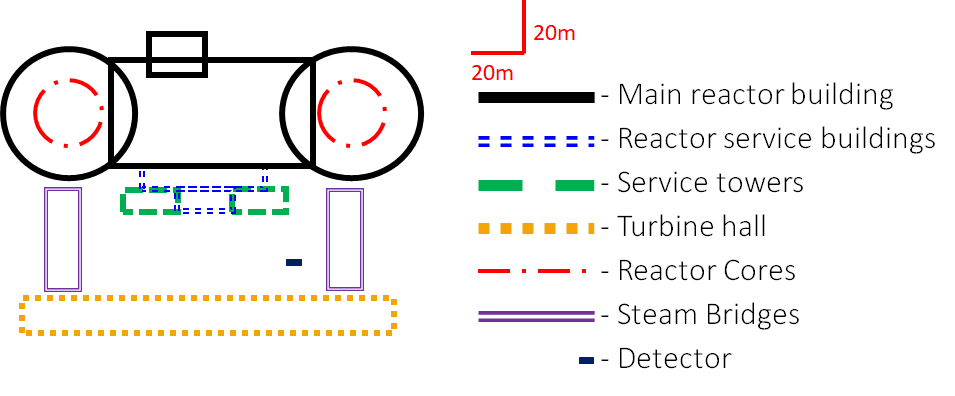
\includegraphics[width=\linewidth]{Chapter5/Figs/wylfaRasterNew/wylfaTraceStep3.png}
%  \captionof{figure}{.} 
%  \label{fig:}
% \end{figure}

\begin{figure}[htbp]
 \centering
 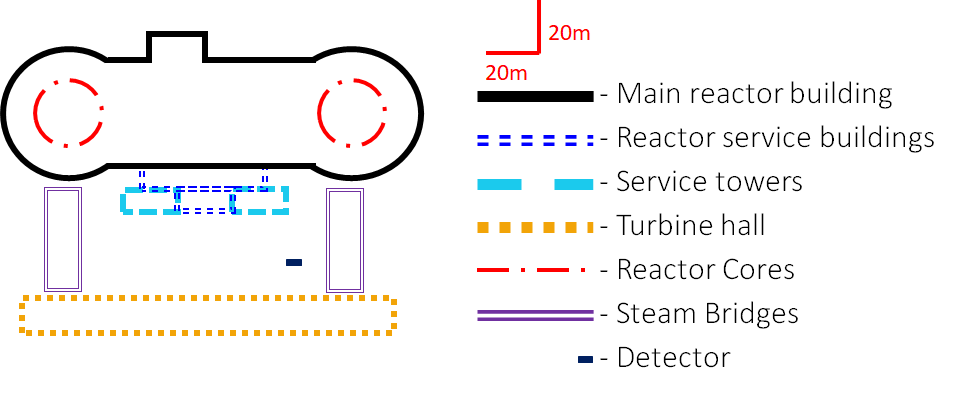
\includegraphics[width=\linewidth]{Chapter5/Figs/wylfaRasterNew/wylfaTraceStep4.png}
 \captionof{figure}{Figure \ref{fig:wylfaTraceStep2} with the overlapping lines and aerial photography from google Earth removed to produce the final trace.}
 \label{fig:wylfaTraceStep4}
\end{figure}

Now that figure \ref{fig:wylfaTraceStep4} has been produced and the features of interest have been identified the cosmic $\mu$ data needs to be analysed. The logic for the track fitter is outlined in section \ref{sec:SimulationOfCosmics} using that tracker the Wylfa data can be fitted an example of which can be seen in figure \ref{fig:3000ExampleEventWithKey}. In figure \ref{fig:3000ExampleEventWithKey} there are many noise events that can potentially cause the fitter to struggle. The tracker however has been custom built around the data set to help prevent any minimisation issues. There are also 3 columns of un-instrumented channels on side A which figure \ref{fig:3000ExampleEventWithKey} shows in grey. These un-instrumented channels inform the fidicual boundaries as well, which figure \ref{fig:3000ExampleEventWithKey} shows too. The number of columns on side A and Side B must be the same otherwise any shadow that the detector will analyse will become distorted in one direction more than the other. Also in figure \ref{fig:3000ExampleEventWithKey} there are a number of dead channels that also have to be carefully considered when assessing tracker performance. By looking at the tracker reconstructed hits on aggregate in figure \ref{fig:wylfaSideABHits} there does not appear to be any bias. In figure \ref{fig:wylfaSideABHits} there are dead channels and channels that fire rarely but there are no areas of low statistics around the dead channels suggesting the tracker is successfully representing the distribution. The only issue is a noisy channel in \ref{subFig:wylfaSideBHits} but as the areas around the channel have statistics comparable to their neighbours its reasonable to assume this is an issue with the channel rather than the fitter. 

\begin{figure}[htbp]
 \centering
 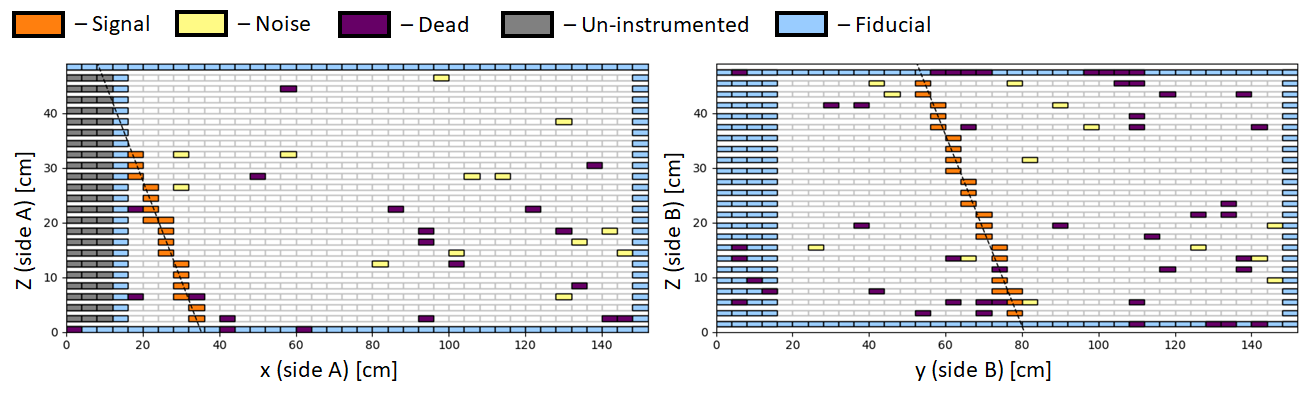
\includegraphics[width=\linewidth]{Chapter5/Figs/wylfaRasterNew/3000ExampleEventWithKey.png}
 \captionof{figure}{A example event from the Wylfa data set with a corresponding key showing how the colour coding relates to the channels. The dashed line represents the fitted line.} 
 \label{fig:3000ExampleEventWithKey}
\end{figure}

\begin{figure}[htbp]
\centering
\begin{subfigure}{.5\textwidth}
  \centering
  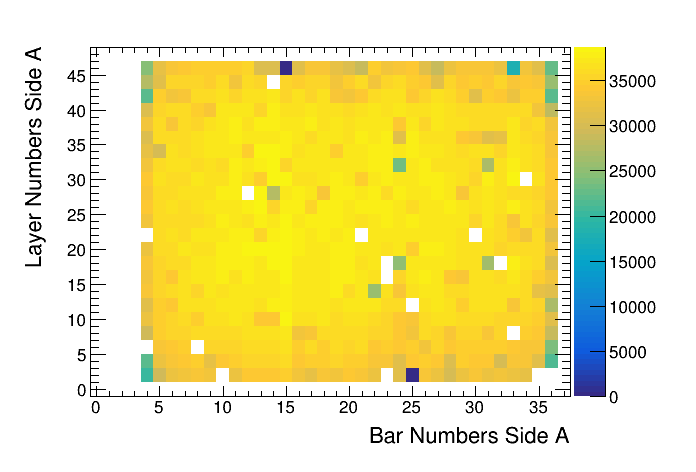
\includegraphics[width=\linewidth]{Chapter5/Figs/wylfaRasterNew/wylfaSideAHits.png}
  \captionsetup{width=.9\linewidth}
  \caption{Bars hit for side A cosmic $\mu$ reconstructed tracks for the Wylfa data set.}
  \label{subFig:wylfaSideAHits}
\end{subfigure}%
\begin{subfigure}{.5\textwidth}
  \centering
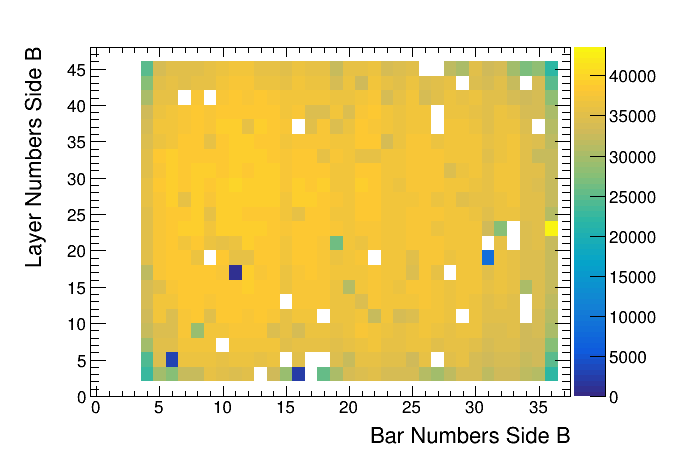
\includegraphics[width=\linewidth]{Chapter5/Figs/wylfaRasterNew/wylfaSideBHits.png}
  \captionsetup{width=.9\linewidth}
  \caption{Bars hit for side B cosmic $\mu$ reconstructed tracks for the Wylfa data set.}
  \label{subFig:wylfaSideBHits}
\end{subfigure}
\caption{Bars hit for sides A and B cosmic $\mu$ reconstructed tracks for the Wylfa data set. The results are mostly even except for a few dead or almost dead channels and one noisy channel on side B. Suggesting the tracker has minimal biasing.}
\label{fig:wylfaSideABHits}
\end{figure}

Once the fitters potential bias has been addressed the $\phi$ and $\theta$ values can be analysed. Due to the high energy and penetrating nature of cosmic $\mu$ \hl{a citation} the reactor buildings may not be dense enough to stop all incoming cosmic $\mu$. As a result the shadows can only be seen with high statistics. However, the detector took cosmic $\mu$ data in accidental coincidence at the Wylfa site and this greatly limited the amount of data that could be gathered to $\sim$ 3 $\times$ 10$^6$ cosmic $\mu$ events. According to the CRY library \cite{ieee_cry_2007} 162000 $\mu^-$ and 174000 $\mu^+$ are produced in 2820\,s for 1 m\,$^2$. VIDARR's top surface area is 1.52\,m $\times$ 1.52\,m = 2.31\,m$^2$ resulting in $\sim$ 275 muons s$^{-1}$. Therefore a data set of 3 $\times$ 10$^6$ cosmic $\mu$ events corresponds to $\sim$ 3 hours of live time. With a rate of 275 muons s$^{-1}$ then the maximum time a fit should be allowed to take is 3600 micro seconds for online track fitting which figure \ref{fig:wylfaTrackerTime} shows is the case for almost all events. Figure \ref{fig:wylfaTrackerTimeLog} takes figure \ref{fig:wylfaTrackerTime} and applies a log to the y axis showing that a very small fraction of events don't fit within the time limit of 3600 micro seconds so a time selection criteria will be required. Whilst online track fitting was not required it is useful to know that the same tracking logic can be applied for both online calibration and full cosmic $\mu$ tomography by only adding a time and $\chi^2$ cut. 

 \begin{figure}[htbp]
 \centering
 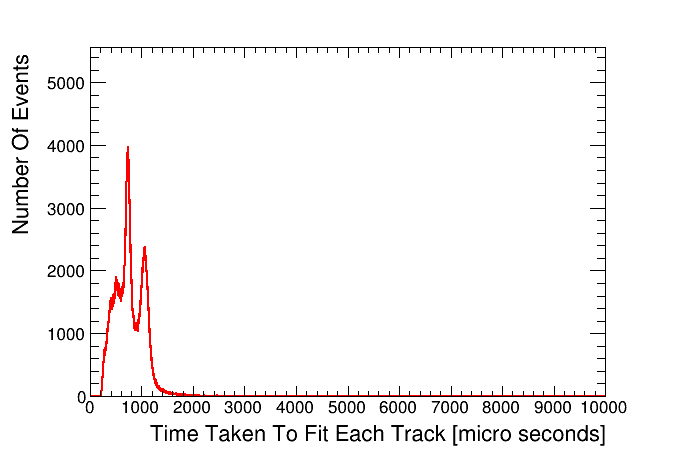
\includegraphics[width=0.7\linewidth]{Chapter5/Figs/Raster/wylfaTrackerTime.png}
 \captionof{figure}{The time taken for each fit for the Wylfa data set. Assuming a rate of $\sim$ 275 cosmic muons s$^{-1}$ then the maximum time allow would be 3600 mirco seconds. Almost all cosmic candidate events fit within this time.} 
 \label{fig:wylfaTrackerTime}
\end{figure}

 \begin{figure}[htbp]
 \centering
 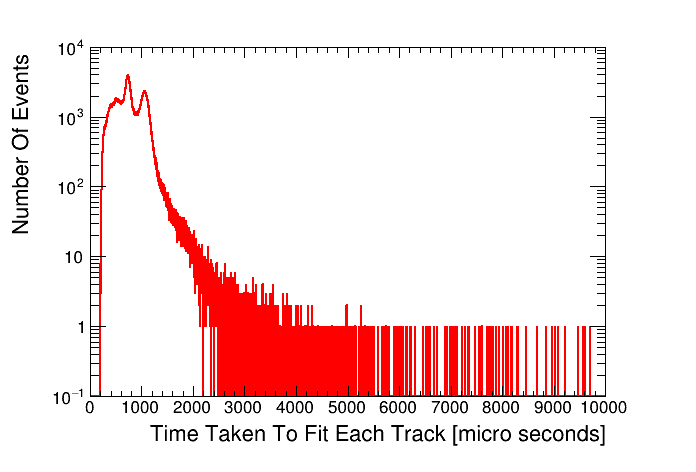
\includegraphics[width=0.7\linewidth]{Chapter5/Figs/Raster/wylfaTrackerTimeLog.png}
 \captionof{figure}{Figure \ref{fig:wylfaTrackerTime} but with the y axis taken as a log some events exceed 3600 micro seconds to fit so a maximum time selection criteria is needed for those events.} 
 \label{fig:wylfaTrackerTimeLog}
\end{figure}

The tracker reconstructed $\phi$ and $\theta$ distribution from the Wylfa data set can be seen in figure \ref{fig:pVsTWylfaReversed} but the shadows don't seem as clear as one would have expected from such dense and heavy buildings. In figure \ref{fig:pVsTWylfaReversed} the bin migration is so significant even though the shadows extend up to 60$^o$ in $\theta$ they are masked very effectively. But the bin migration does become less pronounced as $\theta$ decreases. As $\theta$ decreases the chance of either side having a vertical track is greatly reduced thus reducing the bin migration. However, this poses a problem as the statistics also decrease with $\theta$ as seen in figure \ref{fig:pVsTWylfaReversed}. So by taking the 2d x projection of figure \ref{fig:pVsTWylfaReversed} from 0$^\circ$ -- 37.5$^\circ$ $\theta$ it is possible to ignore most of the bin migration whilst also having suitable statistics to observe the widths of the turbine hall and reactor building which is done in figure \ref{fig:LinearHist_theta_0-37.5_Deg}. It is possible to then take the linear projection in figure \ref{fig:LinearHist_theta_0-37.5_Deg} and then apply it to a circular projection and overlay that projection on top of the wylfa trace seen in figure \ref{fig:wylfaTraceStep4} which is done in figure \ref{fig:wylfaCircular0-37.5Deg_Overlay}. 

 \begin{figure}[htbp]
 \centering
 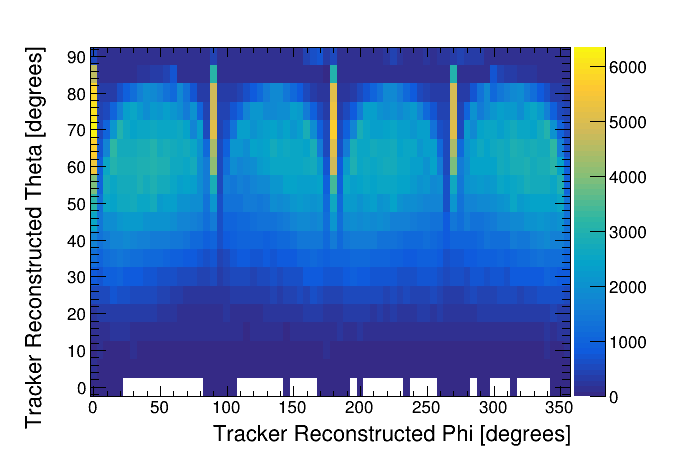
\includegraphics[width=0.7\linewidth]{Chapter5/Figs/Raster/pVsTWylfaReversed.png}
 \captionof{figure}{The cosmic $\mu$ distribution from VIDARR prototype deployment at Wylfa the shadows extend from $\theta$ = 0$^\circ$ -- $\theta$ = 60$^\circ$. Bin migration causes signifficant warping.} 
 \label{fig:pVsTWylfaReversed}
\end{figure}

%  \begin{figure}[htbp]
%  \centering
%  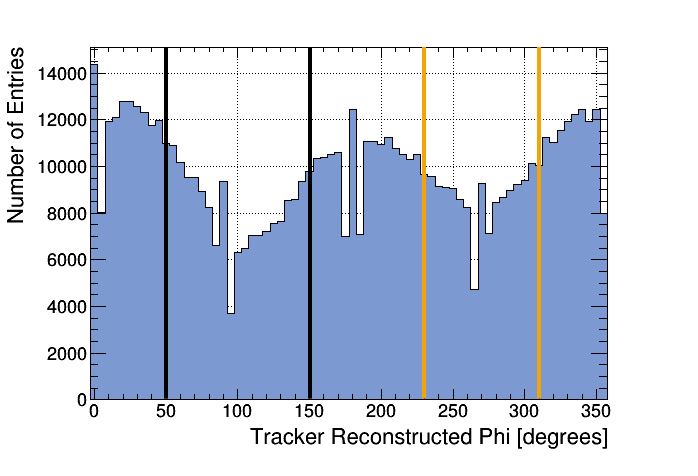
\includegraphics[width=0.7\linewidth]{Chapter5/Figs/wylfaRasterNew/LinearHist_theta_0-57.5_Deg.png}
%  \captionof{figure}{.} 
%  \label{fig:}
% \end{figure}

%  \begin{figure}[htbp]
%  \centering
%  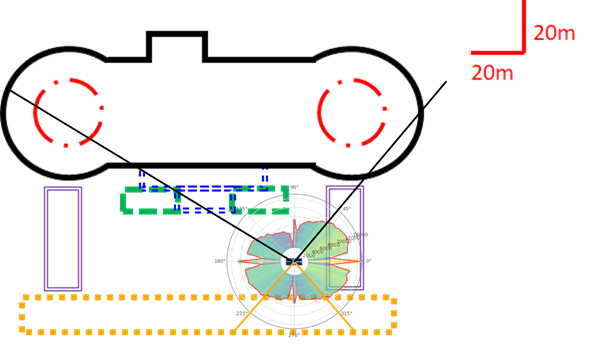
\includegraphics[width=\linewidth]{Chapter5/Figs/wylfaRasterNew/wylfaCircular0-57.5Deg_Overlay.png}
%  \captionof{figure}{.} 
%  \label{fig:}
% \end{figure}

\begin{figure}[htbp]
 \centering
 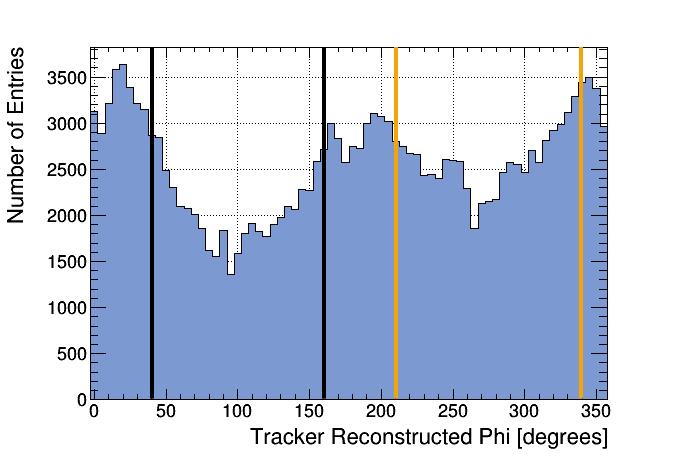
\includegraphics[width=0.7\linewidth]{Chapter5/Figs/wylfaRasterNew/LinearHist_theta_0-37.5_Deg.png}
 \captionof{figure}{Linear histogram showing a 2d projection of figure \ref{fig:pVsTWylfaReversed} from $\theta$ = 0$^\circ$ -- $\theta$ = 37.5$^\circ$ this range was chosen to avoid as much bin migration as possible whilst having as high statistics as possible. The main reactor shadow is highlighted by black lines the turbine hall highlighted by orange lines.}
 \label{fig:LinearHist_theta_0-37.5_Deg}
\end{figure}

 \begin{figure}[htbp]
 \centering
 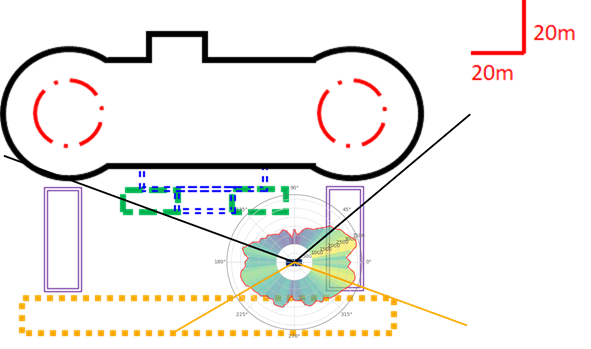
\includegraphics[width=\linewidth]{Chapter5/Figs/wylfaRasterNew/wylfaCircular0-37.5Deg_Overlay.png}
 \captionof{figure}{Figure \ref{fig:wylfaTraceStep4} overlaid with the circular histogram from figure \ref{fig:LinearHist_theta_0-37.5_Deg} to show how the boarders line up with the Wylfa trace.} 
 \label{fig:wylfaCircular0-37.5Deg_Overlay}
\end{figure}

Figure \ref{fig:wylfaCircular0-37.5Deg_Overlay} also shows the limitation of this method. Whilst there are several buildings that should block incident cosmic $\mu$ only the largest building and closest building are visible. Further the far edge of the turbine hall is not clear in figure \ref{fig:wylfaCircular0-37.5Deg_Overlay} even though it should be. This is due to the composition of the turbine hall being corrugated steel (\hl{is there a citation?}) thus blocking fewer cosmic $\mu$. The results from figures \ref{fig:pVsTWylfaReversed} -- \ref{fig:wylfaCircular0-37.5Deg_Overlay} match closely to what we expected to see as figure \ref{fig:sideBySideComparisonTopDownCirc} shows. 

 \begin{figure}[htbp]
 \centering
 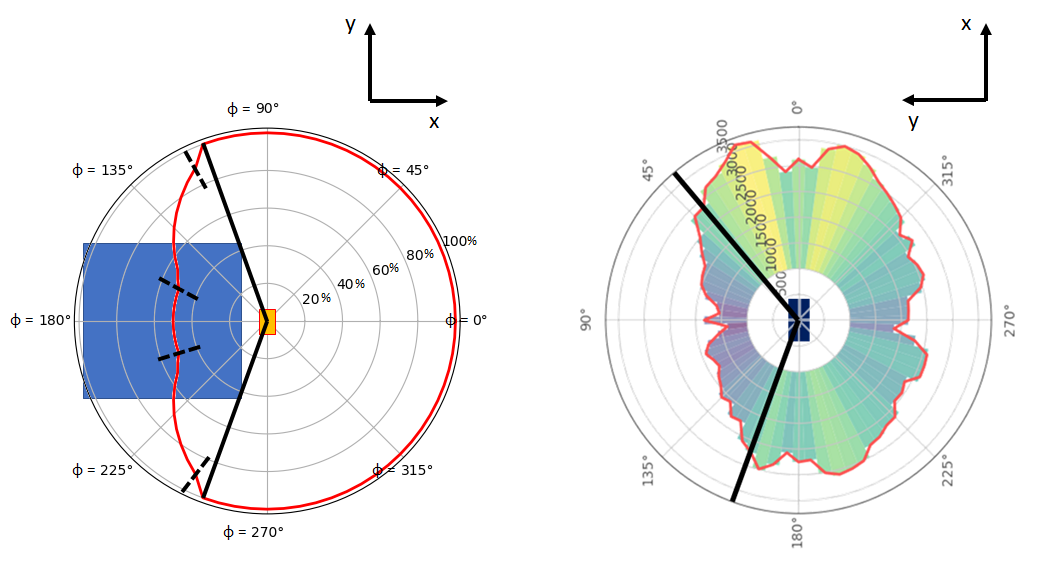
\includegraphics[width=\linewidth]{Chapter5/Figs/wylfaRasterNew/sideBySideComparisonTopDownCirc.png}
 \captionof{figure}{How the circular Wylfa histogram compares to a basic expectation the large tails are visible in both producing a similar shape.}
 \label{fig:sideBySideComparisonTopDownCirc}
\end{figure}

A way to solve the issue of bin migration was highlighted in section \ref{sec:cosMuOverview} which is to use the transmission method as used by the MU-RAY collaboration in figure \ref{fig:mtVesuviusMuRayTransmission} \cite{Ambrosino_2014}. In order for this to work  another data set that reconstructs the whole hemisphere in $\phi$ and $\theta$ is required. It might be possible to use simulated cosmic data to achieve this result however it won't take into account the atmospheric scattering properly (\hl{a couple plots showing this would be nice}). The best approach would be to use measured data in the same location after the demolition of the Wylfa buildings but as that will take decades that is infeasible. Instead measured data was taken at Liverpool from 2016 -- 2018 which produced figure \ref{fig:pVsTLiverpoolReversed}. There are some shadows in the Liverpool data specifically from the accelerator hall at low angles of $\theta$ from 0$^\circ$ -- 17.5 $^\circ$ which is shown in figure \ref{fig:liverpoolShadows}. However once those angles are removed from the data set it serves as a useful control data set as there is minimal cosmic $\mu$ sky blockage. When checking for any potential bias in the Liverpool data set none is visible in either side as shown in figure \ref{fig:liverpoolSideABHits}. 

\begin{figure}[htbp]
 \centering
 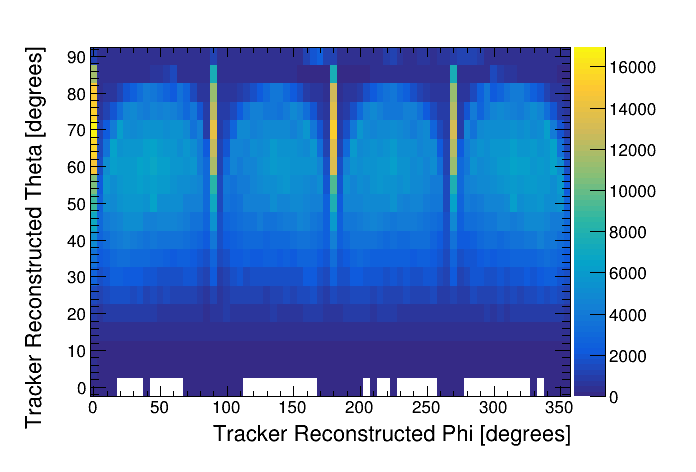
\includegraphics[width=0.7\linewidth]{Chapter5/Figs/Raster/pVsTLiverpoolReversed.png}
 \captionof{figure}{The cosmic $\mu$ distribution from VIDARR prototype deployment at Liverpool the shadows there are some faint shadows below 17.5$^\circ$ but otherwise the data has no major cosmic $\mu$ sky blockage.} 
 \label{fig:pVsTLiverpoolReversed}
\end{figure}

\begin{figure}[htbp]
 \centering
 \includegraphics[width=0.7\linewidth]{Chapter5/Figs/Raster/liverpoolShadows.png}
 \captionof{figure}{The shadows in the Liverpool data below $\theta$ 17.5$^\circ$. The accelerator Hall causes significant cosmic $\mu$ blockage.} 
 \label{fig:liverpoolShadows}
\end{figure}

\begin{figure}[htbp]
\centering
\begin{subfigure}{.5\textwidth}
  \centering
  \includegraphics[width=\linewidth]{Chapter5/Figs/wylfaRasterNew/liverpoolSideAHits.png}
  \captionsetup{width=.9\linewidth}
  \caption{Bars hit for side A cosmic $\mu$ reconstructed tracks for the Liverpool data set.}
  \label{subFig:liverpoolSideAHits}
\end{subfigure}%
\begin{subfigure}{.5\textwidth}
  \centering
\includegraphics[width=\linewidth]{Chapter5/Figs/wylfaRasterNew/liverpoolSideBHits.png}
  \captionsetup{width=.9\linewidth}
  \caption{Bars hit for side B cosmic $\mu$ reconstructed tracks for the Liverpool data set.}
  \label{subFig:liverpoolSideBHits}
\end{subfigure}
\caption{Bars hit for sides A and B cosmic $\mu$ reconstructed tracks for the Liverpool data set. The results are mostly even except for a few dead or almost dead channels and one noisy channel on side B. Suggesting the tracker has minimal biasing.}
\label{fig:liverpoolSideABHits}
\end{figure}

When taking figure \ref{fig:pVsTWylfaReversed} (the Wylfa data) and dividing it by figure \ref{fig:pVsTLiverpoolReversed} (the Liverpool data) and normalising the Liverpool data set to the Wylfa data set and removing the values below 17.5$^\circ$ $\theta$ figure \ref{fig:measuredTrackerReconNoLines} is produced. The shadows are now clearly visible in both $\phi$ and $\theta$ with the main reactor buildings centring around 90$^\circ$ $\phi$ and the turbine hall centring around 270$^\circ$ $\phi$. There are several interesting features seen in figure \ref{fig:measuredTrackerReconNoLines} the top of the turbine hall seen between $\sim$ 240$^\circ$ $\phi$ -- 330$^\circ$ $\phi$ is not well resolved. This is because the turbine hall is made from corrugated steel (\hl{a citation}) and so blocks fewer cosmic $\mu$ and so a significant portion of the building have to be traversed through before the top is visible. But the area from 0$^\circ$ $\phi$ -- 180 $^\circ$ $\phi$ is of particular interest this area contains the main reactor building but also several others. As a result of multiple buildings blocking the path of incident cosmic $\mu$ between the detector and reactor building the shadow patterns are much more complex than one would expect. In addition there appears to be an area of high density between 60$^\circ$ $\phi$ -- 80$^\circ$ $\phi$ and 20$^\circ$ $\theta$ -- 25$^\circ$ $\theta$ which could be the reactor core. In order to determine which components of the shadow are caused by which buildings a simulation is required which has the reactor buildings.

\begin{figure}[htbp]
 \centering
 \includegraphics[width=\linewidth]{Chapter5/Figs/wylfaRasterNew/measuredTrackerReconNoLines.png}
 \captionof{figure}{The measured building shadows taking a ratio of the Wylfa and Liverpool data sets with the Liverpool data acting as a control data set assuming minimal shadows are present in the Liverpool data above 17.5$^\circ$ $\theta$.} 
 \label{fig:measuredTrackerReconNoLines}
\end{figure}

The simulation previously mentioned in chapter \ref{chp:geant4Simulation} has the detector as the centre of the simulation world in the $x$ and $y$ and put the detector on the floor at  $z = 0 $. As such all of the reactor buildings need to be positioned relative to the detector and also placed at $z = 0$. The Wylfa trace seen in figure \ref{fig:wylfaTraceStep4} can be approximated by having certain simple shapes placed on top of the trace as seen in figure \ref{fig:simulatedPositions} which also shows the positions in $x$ and $y$ relative to the detector. Then this can also be done for the widths and depths of the buildings as well shown in figure \ref{fig:simulatedWidthsDepths}. Finally the heights have to be approximated which is done by adjusting the simulated heights until the heights in figure \ref{fig:simulatedHeights} are produced.

 \begin{figure}[htbp]
 \centering
 \includegraphics[width=\linewidth]{Chapter5/Figs/wylfaRasterNew/simulatedPositions.png}
 \captionof{figure}{Positions from the Wylfa trace (figure \ref{fig:wylfaTraceStep4}) with their x and y positions labelled these were then put into GEANT4.} 
 \label{fig:simulatedPositions}
\end{figure}

\begin{figure}[htbp]
 \centering
 \includegraphics[width=\linewidth]{Chapter5/Figs/wylfaRasterNew/simulatedWidthsDepths.png}
 \captionof{figure}{Widths and depths from the Wylfa trace (figure \ref{fig:wylfaTraceStep4}) with their widths and depths labelled these were then put into GEANT4.} 
 \label{fig:simulatedWidthsDepths}
\end{figure}

\begin{figure}[htbp]
 \centering
 \includegraphics[width=\linewidth]{Chapter5/Figs/wylfaRasterNew/simulatedHeights.png}
 \captionof{figure}{Heights estimated from the measured data at Wylfa (figure \ref{fig:pVsTWylfaReversed}) these were then put into GEANT4.} 
 \label{fig:simulatedHeights}
\end{figure}

Figure \ref{fig:WylfaSimGeom_SideOn_TopDown} shows how the simulated geometry looks in  GEANT4. The side on view can be seen in figure \ref{subFig:WylfaSimGeomSideOn} which has the heights annotated and the top down view can be seen in figure \ref{subFig:WylfaSimGeomTopDown} which looks similar to figure \ref{fig:simulatedPositions}. Once these dimensions have been approximate it is possible to simulate both with and without buildings which is done in figure
\ref{fig:thetaVsPhiSimulatedWithReactor_0-100} which shows how the bin migration effects compare with shadows. In simulation the buildings were simulated as 100\,\% concrete, this was done so they would block as many cosmic $\mu$ as possible to give accurate building outlines. Then as with \ref{fig:measuredTrackerReconNoLines} the ratio of the data with and without buildings is also taken  producing figure \ref{fig:simulatedTrackerReconNoLines}. 

\begin{figure}[htbp]
\centering
\begin{subfigure}{.5\textwidth}
  \centering
  \includegraphics[width=\linewidth]{Chapter5/Figs/wylfaRasterNew/WylfaSimGeomSideOn.png}
  \captionsetup{width=.9\linewidth}
  \caption{Simulated geometry in GEANT4 side on perspective.}
  \label{subFig:WylfaSimGeomSideOn}
\end{subfigure}%
\begin{subfigure}{.5\textwidth}
  \centering
\includegraphics[width=\linewidth]{Chapter5/Figs/wylfaRasterNew/WylfaSimGeomTopDown.png}
  \captionsetup{width=.9\linewidth}
  \caption{Simulated geometry in GEANT4 top down perspective.}
  \label{subFig:WylfaSimGeomTopDown}
\end{subfigure}
\caption{The simulated geometry in GEANT4 with heights annotated.}
\label{fig:WylfaSimGeom_SideOn_TopDown}
\end{figure}

\begin{figure}[htbp]
\centering
\begin{subfigure}{.5\textwidth}
  \centering
  \includegraphics[width=\linewidth]{Chapter5/Figs/wylfaRasterNew/thetaVsPhiSimulatedWithReactor0.png}
  \captionsetup{width=.9\linewidth}
  \caption{Simulated $\phi$ and $\theta$ with no reactor buildings and a realistic $\theta$ distribution only bin migration effects are present.}
  \label{subFig:thetaVsPhiSimulatedWithReactor0}
\end{subfigure}%
\begin{subfigure}{.5\textwidth}
  \centering
\includegraphics[width=\linewidth]{Chapter5/Figs/wylfaRasterNew/thetaVsPhiSimulatedWithReactor100.png}
  \captionsetup{width=.9\linewidth}
  \caption{Simulated $\phi$ and $\theta$ with reactor buildings that are 100\,\% concrete and a realistic $\theta$ distribution.}
  \label{subFig:thetaVsPhiSimulatedWithReactor100}
\end{subfigure}
\caption{A side by side comparison of the GEANT4 simulation with and without reactor buildings using a realistic $\theta$ distribution.}
\label{fig:thetaVsPhiSimulatedWithReactor_0-100}
\end{figure}

\begin{figure}[htbp]
 \centering
 \includegraphics[width=\linewidth]{Chapter5/Figs/wylfaRasterNew/simulatedTrackerReconNoLines.png}
 \captionof{figure}{The simulated building shadows taking the ratio with reactor buildings and without reactor buildings highlighting the composite shadow shapes.} 
 \label{fig:simulatedTrackerReconNoLines}
\end{figure}

Using the GEANT4 simulation it is possible to simulate each building and outline each one which can then be overlaid on top of figure \ref{fig:simulatedTrackerReconNoLines} to produce figure \ref{fig:simulatedTrackerRecon} which uses the same outline styles as figure \ref{fig:wylfaTraceStep4}. Then its possible take those outlines and overlap them on top of the measured shadows from the Wylfa reactor site in figure \ref{fig:measuredTrackerReconNoLines} to produce figure \ref{fig:measuredTrackerRecon}. In figure \ref{fig:measuredTrackerRecon} we can see that the overall outlines match up reasonably well with the measured data. It is also possible to overlay these results using a circular top down plot as well which is done in figure \ref{fig:wylfaCircular0-37.5Deg_Overlay_Updated}. By doing this it is possible to show that the area of high density viewed in figure \ref{fig:measuredTrackerRecon} is most likely the reactor core as it lines up with expectations of where the near reactor core is. 

\begin{figure}[htbp]
 \centering
 \includegraphics[width=\linewidth]{Chapter5/Figs/wylfaRasterNew/simulatedTrackerRecon.png}
 \captionof{figure}{Figure \ref{fig:simulatedTrackerReconNoLines} with each simulated reactor building highlighted using lines which correspond to the key in \ref{fig:wylfaTraceStep4}.} 
 \label{fig:simulatedTrackerRecon}
\end{figure}

\begin{figure}[htbp]
 \centering
 \includegraphics[width=\linewidth]{Chapter5/Figs/wylfaRasterNew/measuredTrackerRecon.png}
 \captionof{figure}{Figure \ref{fig:measuredTrackerReconNoLines} with each simulated reactor building highlighted using lines which correspond to the key in \ref{fig:wylfaTraceStep4}.} 
 \label{fig:measuredTrackerRecon}
\end{figure}

\begin{figure}[htbp]
 \centering
 \includegraphics[width=\linewidth]{Chapter5/Figs/wylfaRasterNew/wylfaCircular0-37.5Deg_Overlay_Updated.png}
 \captionof{figure}{An updated version of figure \ref{fig:wylfaCircular0-37.5Deg_Overlay} using the boundaries from the Wylfa trace (figure \ref{fig:wylfaTraceStep4}) and figure \ref{fig:measuredTrackerRecon}. To highlight the key features of the turbine hall main reactor building and reactor core.}  
 \label{fig:wylfaCircular0-37.5Deg_Overlay_Updated}
\end{figure}

\section{Cosmic Tracker Uncertainties}\label{sec:cosmicTrackerUncertainties}
The cosmic $\mu$ results from figures \ref{fig:simulatedTrackerRecon} \ref{fig:measuredTrackerRecon} and \ref{fig:wylfaCircular0-37.5Deg_Overlay_Updated} are highly promising. However, there are some potential issues with regards to the bin migration previously mentioned especially in figures \ref{fig:measuredTrackerReconNoLines} and \ref{fig:measuredTrackerRecon} where the vertical lines at $\phi$ = 0$^\circ$, $\phi$ = 90$^\circ$, $\phi$ = 180$^\circ$, $\phi$ = 270$^\circ$ are still visible. The uncertainties can be quantified to some extent, but the limits are more due to the detector's geometry and segmentation. In order to quantify the uncertainty of the tracker and detector 1E6 particles were simulated in GEANT4 with a $\phi$ =  135$^\circ$ and $\theta$ = 45$^\circ$ a random spot is then chosen in the detector and then they are back projected by 3\,m. The generated distribution of which can be seen in figure \ref{fig:sideABGen_PVsT_135_45}. The fitter then reconstructs the tracks shown in figure \ref{fig:trackedABWithDead}. When comparing the tracker results from figure \ref{fig:trackedABWithDead} with the generated distributions in figure \ref{fig:sideABGen_PVsT_135_45} there is minimal difference which is unsurprising as the efficiency is 98.6\,\% for the reconstruction. 

\begin{figure}[htbp]
\centering
\begin{subfigure}{.5\textwidth}
  \centering
  \includegraphics[width=\linewidth]{Chapter5/Figs/cosmicTrackerUncertainties/sideAGen_PVsT_135_45.png}
  \captionsetup{width=.9\linewidth}
  \caption{Side A generated hits for $\phi$ =  135$^\circ$ and $\theta$ = 45$^\circ$.}
  \label{subFig:sideAGen_PVsT_135_45}
\end{subfigure}%
\begin{subfigure}{.5\textwidth}
  \centering
\includegraphics[width=\linewidth]{Chapter5/Figs/cosmicTrackerUncertainties/sideBGen_PVsT_135_45.png}
  \captionsetup{width=.9\linewidth}
  \caption{Side B generated hits for $\phi$ = 135$^\circ$ and $\theta$ = 45$^\circ$.}
  \label{subFig:sideBGen_PVsT_135_45}
\end{subfigure}
\caption{The generated hits in GEANT4 for $\phi$ = 135$^\circ$ and $\theta$ = 45$^\circ$ with dead and un-instrumented channels taken into account.}
\label{fig:sideABGen_PVsT_135_45}
\end{figure}

\begin{figure}[htbp]
\centering
\begin{subfigure}{.5\textwidth}
  \centering
  \includegraphics[width=\linewidth]{Chapter5/Figs/cosmicTrackerUncertainties/trackedAWithDead.png}
  \captionsetup{width=.9\linewidth}
  \caption{Side A tracker reconstructed hits for $\phi$ = 135$^\circ$ and $\theta$ = 45$^\circ$.}
  \label{subFig:trackedAWithDead}
\end{subfigure}%
\begin{subfigure}{.5\textwidth}
  \centering
\includegraphics[width=\linewidth]{Chapter5/Figs/cosmicTrackerUncertainties/trackedBWithDead.png}
  \captionsetup{width=.9\linewidth}
  \caption{Side B tracker reconstructed hits for $\phi$ = 135$^\circ$ and $\theta$ = 45$^\circ$.}
  \label{subFig:trackedBWithDead}
\end{subfigure}
\caption{Tracker reconstructed hits for the $\phi$ 135$^\circ$ and $\theta$ = 45$^\circ$ the tracker is not thrown off by the dead channels or the fiducial channels. It reconstructs the simulated distribution well.}
\label{fig:trackedABWithDead}
\end{figure}

The reconstructed $\phi$ and $\theta$ that the tracker produces is shown in figure \ref{fig:pVsTWithDeadLog} where about $\sim$ 50\,\% of the data is reconstructed to 135$^\circ$ 45$^\circ$ bin. However, in figure \ref{fig:pVsTWithDeadLog} there is significant smearing in both angles. The smearing in $\phi$ is roughly even with smearing likely to be both above and below the generated value of $\phi$ = 135$\circ$. More interesting is the smearing in $\theta$ which is more likely to smear above the generated value than below of $\theta$ = 45$^\circ$. This is a result of how cosmic $\mu$ events propagate in the detector and the nature of fiducialisation in the detector. In figure \ref{fig:badFitNoFiducial} an example event shows how the fitter ignores noise and fits signal. But figure \ref{fig:badFitWithFiducial} shows how that can become a problem once the detector is made narrower the noise is now being treated as part of the cosmic $\mu$ event. This has had the effect of pushing the event to a higher value of $\theta$ and a lower value of $\phi$. Even if the noise is properly excluded as in figure \ref{fig:badFitNoFiducial} there isn't enough information to correctly extrapolate the correct values of $\phi$ and $\theta$ as the event in \ref{fig:badFitWithFiducial} is only 2 channels wide. Also due to timing and electronic effects sometimes cosmic $\mu$ events will have large gaps inside of them in real world data so excluding events like \ref{fig:badFitWithFiducial} is not feasible. As cosmic $\mu$ events propagate downwards through the detector the fitter will be more likely the fitter will fit above expected values rather than below as corner clipping events are likely to be narrower than the $\mu$ even they represent this is also a key component of the bin migration previously mentioned. 

\begin{figure}[htbp]
 \centering
 \includegraphics[width=\linewidth]{Chapter5/Figs/cosmicTrackerUncertainties/pVsTWithDeadLog.png}
 \captionof{figure}{Tracker reconstructed $\phi$ and $\theta$ for simulated $\phi$ = 135$^\circ$ and $\theta$ = 45$^\circ$. The most likely value to be reconstructed is $\phi$ = 135$^\circ$ and $\theta$ = 45$^\circ$ (representing $\sim$ 55\,\% of the reconstruction) but there is significant smearing in both angles. But efficiency is 98.6\,\%.} 
 \label{fig:pVsTWithDeadLog}
\end{figure}

\begin{figure}[htbp]
 \centering
 \includegraphics[width=\linewidth]{Chapter5/Figs/cosmicTrackerUncertainties/135,45_85,60__noDead_updatedAxis_cosmicCandidate195939.png}
 \captionof{figure}{Example candidate cosmic event from the generated GEANT4 data for $\phi$ = 135$^\circ$ and $\theta$ = 45$^\circ$ with all channels. The tracker correctly ignores the noise and fits the signal.} 
 \label{fig:badFitNoFiducial}
\end{figure}

\begin{figure}[htbp]
 \centering
 \includegraphics[width=\linewidth]{Chapter5/Figs/cosmicTrackerUncertainties/135,45_85,60__withDead_updatedAxis_cosmicCandidate195939.png}
 \captionof{figure}{figure \ref{fig:badFitNoFiducial} with fiducial dead and un-instrumented channels taken into account. The tracker tries to fit the signal but due to corner clipping nature of the event the fitting on side A has failed and fits to $\phi$ = 85$^\circ$ and $\theta$ = 60$^\circ$ instead of $\phi$ = 135$^\circ$ and $\theta$ = 45$^\circ$. } 
 \label{fig:badFitWithFiducial}
\end{figure}

Fitting both $\phi$ and $\theta$ yields bad results which is unsurprising considering how significant the smearing is in figure \ref{fig:pVsTWithDeadLog}. For both the $\chi^2$/DOF is > 170 which is far above acceptable levels (see figures \ref{fig:fittingPhiWithDead}, \ref{fig:fittingThetaWithDead}). In both cases the function attempted to be fitted is a double Gaussian function with a ``noise'' Gaussian function to take into account the smearing and a Gaussian attempting to fit the signal. For $\phi$ the signal mean was 136.288$^\circ$ and the signal $\sigma$ was 0.728$^\circ$. Considering the spread on $\phi$ is significant these values are reasonable but its clear from figure \ref{fig:fittingPhiWithDead} that the top of the signal distribution isn't being fitted well. For $\theta$ the signal mean was 45.1275$^\circ$ and the signal $\sigma$ was 0.3524$^\circ$. These values are very good for $\theta$ and whilst the fit has large $\chi^2$/DOF in figure \ref{fig:fittingThetaWithDead} the signal distribution seems to have been fitted quite well. It is not surprising that the fitting for $\theta$ is more accurate as the segments for the detector are 4 times wider than they are tall. 

\begin{figure}[htbp]
 \centering
 \includegraphics[width=\linewidth]{Chapter5/Figs/cosmicTrackerUncertainties/fittingPhiWithDead.png}
 \captionof{figure}{Double Gaussian fitted to the reconstructed tracker $\phi$ values when simulating $\phi$ = 135$^\circ$ and $\theta$ = 45$^\circ$ exclusively. The $\chi^2$/DOF is 181.31 showing a poor fit which is largely due to segmentation effects. signal mean = 136.288, signal $\sigma$ 0.728, noise mean = 140.101, noise $\sigma$ 7.819.} 
 \label{fig:fittingPhiWithDead}
\end{figure}

\begin{figure}[htbp]
 \centering
 \includegraphics[width=\linewidth]{Chapter5/Figs/cosmicTrackerUncertainties/fittingThetaWithDead.png}
 \captionof{figure}{Double Gaussian fitted to the reconstructed tracker $\theta$ values when simulating $\phi$ = 135$^\circ$ and $\theta$ = 45$^\circ$ exclusively. The $\chi^2$/DOF is 172.758 showing a poor fit which is largely due to segmentation effects. Signal mean = 45.1275, signal $\sigma$ = 0.3524, noise mean = 46.8153, noise $\sigma$ = 1.6294.} 
 \label{fig:fittingThetaWithDead}
\end{figure}

It is possible to mitigate the effect of these corner clipping events by requiring a large number of bar segments to be hit per side. In figure \ref{fig:pVsT135FidFix_20barCutPerSide} a requirement of 20 bars being hit for each side is introduced. When comparing figure \ref{fig:pVsTWithDeadLog} which requires 4 bars to be hit per side and figure \ref{fig:pVsT135FidFix_20barCutPerSide} which requires 20 bars to be hit per side the spread has been greatly reduced. However this selection criteria reduces the efficiency from 98.6\,\% to 68.9\,\%. But this effect does not effect all events equally, events with a lower value of $\theta$ will be more likely to be removed. As a result when using this selection criteria on the measured data in figure \ref{fig:20CutRatioWylfaDivLiv} the shadows become less clear as $\theta$ decreases. This highlights the paradox between increasing precision and increasing accuracy for this particular data set. Cosmic $\mu$ events that cross the corner of the detector are the most useful for cosmic $\mu$ tomography at low angles of $\theta$ so shadow analysis that uses these events will be more accurate. But these are also the events that will have the most smearing and so will have less precision. 

\begin{figure}[htbp]
 \centering
 \includegraphics[width=\linewidth]{Chapter5/Figs/cosmicTrackerUncertainties/pVsT135FidFix_20barCutPerSide.png}
 \captionof{figure}{Figure \ref{fig:pVsTWithDeadLog} but with all events that have $<$ 20 hits for side A and $<$ 20 hits for side B removed. This greatly improves the distribution and reduces smearing. However efficiency is only 68.9\,\% $\sim$ 30\,\% lower than with a 4 bar cut either side.} 
 \label{fig:pVsT135FidFix_20barCutPerSide}
\end{figure}

\begin{figure}[htbp]
 \centering
 \includegraphics[width=\linewidth]{Chapter5/Figs/cosmicTrackerUncertainties/20CutRatioWylfaDivLiv.png}
 \captionof{figure}{How the ratio of the Liverpool and Wylfa data sets looks when a 20 bar cut per side is used. Instead of a 4 bar cut (See figures \ref{fig:measuredTrackerReconNoLines} and \ref{fig:measuredTrackerRecon}). The shadows for both the turbine hall (centred around $\phi$ = 270$^\circ$) and reactor buildings (centred around $\phi$ = 90 $^\circ$) are less accurately resolved now. Despite the more accurate angle reconstruction the number of side on events has been greatly reduced and as those are the most useful events for this tomography the outlines have greatly degraded. \hl{This plot needs to be redone to match the others like it}.}
 \label{fig:20CutRatioWylfaDivLiv}
\end{figure}

\section{Using Simulated Data as Control Data}
Another possible alternative to using the Liverpool data set as a control data set is to use simulated data as a control data set. However, this has major limitations even when using a $\theta$ distribution which is derived from measured data (\hl{probably better to use CRY distribution}). The overall $\theta$ distribution for simulated data can be seen in figure \ref{fig:mc_thetaOnly} which is a good approximation to the measured data in figure \ref{fig:measuredThetaWylfaLiverpool}. The overall $\phi$ and $\theta$ distribution for the simulated data can be seen in figure \ref{fig:mc_PvsT} providing the $\theta$ distribution is accurate and the GEANT4 simulation correctly models the atmospheric smearing this should only have detector effects and segmentation effects smearing the distribution. 

\begin{figure}[htbp]
 \centering
 \includegraphics[width=0.7\linewidth]{Chapter5/Figs/UsingSimulatedDataAsControl/mc_theatOnly.png}
 \captionof{figure}{$\theta$ distribution from simulation using measured data and redistributing to account for potential reconstruction issues and using an exponential tail fit. \hl{plot needs to be reversed and need to use CRY distribution}}
 \label{fig:mc_thetaOnly}
\end{figure}

\begin{figure}[htbp]
\centering
\begin{subfigure}{.5\textwidth}
  \centering
  \includegraphics[width=\linewidth]{Chapter5/Figs/UsingSimulatedDataAsControl/measuredThetaWylfa.png}
  \captionsetup{width=.9\linewidth}
  \caption{The tracker reconstructed $\theta$ distribution for Wylfa cosmic $\mu$ events.}
  \label{subFig:measuredThetaWylfa}
\end{subfigure}%
\begin{subfigure}{.5\textwidth}
  \centering
\includegraphics[width=\linewidth]{Chapter5/Figs/UsingSimulatedDataAsControl/measuredThetaLiverpool.png}
  \captionsetup{width=.9\linewidth}
  \caption{The tracker reconstructed $\theta$ distribution for Liverpool cosmic $\mu$ events.}
  \label{subFig:measuredThetaLiverpool}
\end{subfigure}
\caption{The measured $\theta$ distributions for Wylfa and Liverpool there's a peak at 60$^\circ$ in both and the overall reconstructed distributions look similar.}
\label{fig:measuredThetaWylfaLiverpool}
\end{figure}

\begin{figure}[htbp]
 \centering
 \includegraphics[width=0.7\linewidth]{Chapter5/Figs/UsingSimulatedDataAsControl/mc_PvsT.png}
 \captionof{figure}{$\phi$ and $\theta$ distribution for simulated data using the distribution for theta seen in figure \ref{fig:mc_thetaOnly}.\hl{plot needs to be reversed and needs to be redone with CRY distribution + reformatting}.}
 \label{fig:mc_PvsT}
\end{figure}

However, the simulation can't quite account for all of the different effects as seen in figure \ref{fig:WylfaToMCRatio} when the ratio is taken between simulation and measured Wylfa data. In figure \ref{fig:WylfaToMCRatio} the bin migration is still obscuring the shadows quite significantly. It is possible to force the ratio plot to be between 0 and 2 which is done in figure \ref{fig:WylfaToMCRatio0-2} when this is done it is possible to see the Wylfa shadows however the bin migration makes it difficult to determine where the shadows for the turbine hall and reactor buildings separate. The same effect can be seen when taking the ratio between GEANT4 and Liverpool data in figures \ref{fig:LiverpoolToMCRatio} \ref{fig:LiverpoolToMCRatio0-2} which clearly shows that the simulated distribution is struggling to act as a control data set. The amount of cosmic $\mu$ sky blockage is very minimal in the Liverpool data set but there is still a large discrepancy between that data set and the generated cosmic $\mu$ data set. As a result the Liverpool data set is the preferred control data set to the generated GEANT4 data. 

\begin{figure}[htbp]
 \centering
 \includegraphics[width=0.7\linewidth]{Chapter5/Figs/UsingSimulatedDataAsControl/WylfaToMCRatio.png}
 \captionof{figure}{Ratio of Wylfa to GEANT4 simulated data the bin migration hides the shadows \hl{Needs to be redone with Cry Distribution + reformatting}} 
 \label{fig:WylfaToMCRatio}
\end{figure}

\begin{figure}[htbp]
 \centering
 \includegraphics[width=0.7\linewidth]{Chapter5/Figs/UsingSimulatedDataAsControl/WylfaToMCRatio0-2.png}
 \captionof{figure}{Ratio of Wylfa to GEANT4 simulated data restricted to a maximum of 2 the bin migration still causes the tops of the shadows to be difficult to determine. \hl{Needs to be redone with Cry Distribution + reformatting}}
 \label{fig:WylfaToMCRatio0-2}
\end{figure}

\begin{figure}[htbp]
 \centering
 \includegraphics[width=0.7\linewidth]{Chapter5/Figs/UsingSimulatedDataAsControl/LiverpoolToMCRatio.png}
 \captionof{figure}{Ratio of Liverpool to GEANT4 simulated data the bin migration dominates \hl{Needs to be redone with Cry Distribution + reformatting}.}
 \label{fig:LiverpoolToMCRatio}
\end{figure}

\begin{figure}[htbp]
 \centering
 \includegraphics[width=0.7\linewidth]{Chapter5/Figs/UsingSimulatedDataAsControl/LiverpoolToMCRatio0-2.png}
 \captionof{figure}{Ratio of the Liverpool to GEANT4 simulated data restricted to a maximum of 2. Unexpected areas below blocked incidence of 1 are visible even though there is nothing at the Liverpool site that could cause such shadows to occur. \hl{Needs to be redone with Cry Distribution + reformatting}.}
 \label{fig:LiverpoolToMCRatio0-2}
\end{figure}

% Cosmic $\mu$ tomography is split into two distinct types two sided and one sided. Two sided cosmic $\mu$ is preferred if it is feasible this is because both attenuation and scattering can be measured when using this technique. The effect of the cosmic $\mu$ scattering can be seen in figure \ref{fig:twoSidedCosmicMuonTomographySchults} the cosmic $\mu$ which travel through the dense object will scatter more than the cosmic $\mu$ that don't. By making coincident measurements of the cosmic $\mu$ it is possible to find vertices using this method. This method is extremely powerful but can only be used for smaller objects in most cases. 
% \\\\ For larger objects one sided cosmic $\mu$ tomography has to be used. An example of what one sided cosmic muon tomography looks like can be seen in figure \ref{fig:oneSidedCosmicMuonExample} when there is an object that can attenuate cosmic $\mu$ then the number of cosmic $\mu$ will decrease in the direction of the object being imaged. This method cannot measure scattering or vertices however that is still sufficient in many cases such as the imaging done by the DIAPHANE collaboration seen in figure  \ref{fig:diaphaneStructualImaging}. Which uses 4 different locations to image the La Soufriere of Guadeloupe dome and measure the density for volcanic observations \cite{Marteau_2017}.
% \\\\Need to cite \cite{ANASTASIO2013423} talking about Mu-Ray and SiPms blah

% In order to find the approximate position of detector at the Wylfa site Google Maps was used as the detector's container was large enough to be seen by the Google Maps satellite. The initial step can be seen in figure \ref{fig:wylfaTraceStep0}. Once the detector position has been identified a rough trace of the buildings is then performed with basic shapes seen in figure \ref{fig:wylfaTraceStep1}. However because the site buildings are taller than the detector by quite a significant margin the base position of the buildings does not match the top position of the buildings seen in the google maps. In figure \ref{fig:wylfaTraceStep2} key areas of the site buildings are used as anchor points to so that the base of the buildings is more accurately represented. Finally the background and any connecting lines are removed in figure \ref{fig:wylfaTraceStep4} which shows the final Wylfa trace.  

% \begin{figure}[htbp]
%  \centering
%  \includegraphics[width=\linewidth]{Chapter5/Figs/Raster/wylfaTraceStep0.png}
%  \captionof{figure}{The detector at the Wylfa reactor site.} 
%  \label{fig:wylfaTraceStep0}
% \end{figure}

% \begin{figure}[htbp]
%  \centering
%  \includegraphics[width=\linewidth]{Chapter5/Figs/Raster/wylfaTraceStep1.png}
%  \captionof{figure}{Basic shapes are overlaid on top of the detector and site buildings.} 
%  \label{fig:wylfaTraceStep1}
% \end{figure}

% \begin{figure}[htbp]
%  \centering
%  \includegraphics[width=\linewidth]{Chapter5/Figs/Raster/wylfaTraceStep2.png}
%  \captionof{figure}{Anchor points are used to offset the tall site buildings closer to the base of the buildings. This is done to take into account the angle of the google maps satellite.} 
%  \label{fig:wylfaTraceStep2}
% \end{figure}

% \begin{figure}[htbp]
%  \centering
%  \includegraphics[width=\linewidth]{Chapter5/Figs/Raster/wylfaTraceStep4.png}
%  \captionof{figure}{Finally the background of the reactor site is removed and we are left with a trace of the reactor site.} 
%  \label{fig:wylfaTraceStep4}
% \end{figure}

% The cosmic $\mu$ tracker has several steps. First if fewer than 8 bars are hit above 0.7\,MeV the event is discarded. Then if either side has less than 4 hits > 0.7\,MeV the event is discarded. Then the top and bottom hit is found for each side of the detector from this a basic approximation of the gradient is found. This provides a starting point for the fitter on each side, this leads to the initial fit where all of the events above the 0.7\,MeV threshold are fitted, this is preferred over clustering as it includes low angled $\theta$ cosmic $\mu$ that clustering often removes. Then any hits that are 2 bars away from the track are discarded, and any lone hits that are 8 bars away from any other hits are also removed then the second fit is applied. Then any hits within one bar of the fitted track are then re-accepted as part of the track. Any lone hits to within a radius of 4 bars from the track are once again removed. This then leads to the third and final fit, which is very fast as the approximation by the second fit is usually quite close to third fit. Then any track which has less than 4 hits per side is then rejected. Finally if 50\,\% of the track energy is missing in either side the event is also removed, this is because under such circumstances it is likely that a second cosmic event is inside the detector or a shower has produced multiple tracks. In figure \ref{fig:3000ExampleEvent} it can be seen that even with a large number of noise hits ($\sim$ 10 noise hits per side) the fitter has still accurately reconstructed the event. 
 
% \begin{figure}[htbp]
%  \centering
%  \includegraphics[width=\linewidth]{Chapter5/Figs/Raster/testEventNewScheme.png}
%  \captionof{figure}{An example event from the Wylfa deployment the cosmic enters through the top of the detector and exits through the bottom. The signal that the tracker has identified is shown in orange. The hits the tracker discards are shown in yellow. The un-instrumented block on side A is shown in grey. The dead channels are shown in dark purple. The channels removed for fiducial purposes are shown in light blue.} 
%  \label{fig:3000ExampleEvent}
% \end{figure}

% Using this fitter the data from both the 2014 -- 2015 Wylfa deployment, figure \ref{fig:pVsTWylfaReversed}, and the 2015 -- 2018 deployment at Liverpool, figure \ref{fig:pVsTLiverpoolReversed}, can be analysed for tomographic purposes. Both of these data sets have shadows in them, the shadows in the Liverpool data set are significantly fainter than the shadows in the Wylfa data as the buildings at Wylfa are mostly comprised of concrete where as the buildings at Liverpool are mostly comprised of brick, glass, and steel. In the Liverpool data set the shadows are only visible at very shallow angles of $\theta$ due to the difference in building densities. At Liverpool whilst other buildings are visible in the data set the old accelerator hall is the most visible component which is highlighted in figure \ref{fig:liverpoolCirShadows}. However these shadows are only visible from 0$^{\circ}$ $\theta$ -- 17.5$^{\circ}$ $\theta$, at angles higher than 17.5 $^{\circ}$ $\theta$ the shadows are too faint. 
% \begin{figure}[htbp]
%  \centering
%  \includegraphics[width=0.8\linewidth]{Chapter5/Figs/Raster/pVsTWylfaReversed.png}
%  \captionof{figure}{Measured $\theta$ and $\phi$ from the cosmic muons from the Wylfa deployment, the reactor is at $\sim$ 90$^{\circ}$. The turbine hall is at $\sim$ 270$^{\circ}$.} 
%  \label{fig:pVsTWylfaReversed}
% \end{figure}

% \begin{figure}[htbp]
%  \centering
%  \includegraphics[width=0.8\linewidth]{Chapter5/Figs/Raster/pVsTLiverpoolReversed.png}
%  \captionof{figure}{Measured $\theta$ and $\phi$ from the cosmic muons from the Liverpool deployment.} 
%  \label{fig:pVsTLiverpoolReversed}
% \end{figure}

% \begin{figure}[htbp]
%  \centering
%  \includegraphics[width=0.8\linewidth]{Chapter5/Figs/Raster/liverpoolShadows.png}
%  \captionof{figure}{Measured $\theta$ and $\phi$ from the cosmic muons from the Liverpool deployment shown with the map of Liverpool in the background. The major dip at highlighted by the black lines is due to the accelerator hall at Liverpool.} 
%  \label{fig:liverpoolCirShadows}
% \end{figure}

% The shadows in the Wylfa data are much clearer, seen in figures \ref{fig:WylfaSlice0-57.5} and \ref{fig:wylfaTraceAbove32.5} shows $\phi$ from 0$^{\circ}$ $\theta$ -- 57.5$^{\circ}$ $\theta$ the shadows are clearly visible from both the turbine hall highlighted in-between the orange lines and the reactor buildings shown in-between the black lines. The shape however does not accurately represent the size of the reactor footprint or the width of the turbine hall. This is due to the angles of cosmic $\mu$ that are being attenuated by the buildings. In order to accurately quantify the width of the reactor building cosmic $\mu$ from lower angles must be considered in figures \ref{fig:WylfaSlice0-37.5} and \ref{fig:wylfaTraceAbove52.5}  show $\phi$ from 0$^{\circ}$ $\theta$ -- 37.5$^{\circ}$ $\theta$ this now gives a much more accurate estimate for the size of the reactor building and $phi$. The size of the turbine hall in $\phi$ is less accurate due to the corrugated steel the turbine hall is constructed with, this means the far edge of the turbine hall is hard to discern which can be seen in figure \ref{fig:wylfaTraceAbove52.5}.

% \begin{figure}[htbp]
% \centering
% \begin{subfigure}{.5\textwidth}
%   \centering
%   \includegraphics[width=\linewidth]{Chapter5/Figs/Raster/linReversedWylfaSlice0-57.5.png}
%   \captionsetup{width=.9\linewidth}
%   \caption{Linear histogram showing the dips in the shadows from the shadows of the reactor buildings and turbine halls.}
%   \label{subFig:linReversedWylfaSlice0-57.5}
% \end{subfigure}%
% \begin{subfigure}{.5\textwidth}
%   \centering
%   \includegraphics[width=0.765\linewidth]{Chapter5/Figs/Raster/cirReversedWylfaSlice0-57.5.png}
%   \captionsetup{width=.9\linewidth}
%   \caption{Circular histogram showing the dips in the shadows from the shadows of the reactor buildings and turbine halls.}
%   \label{subFig:linReversedWylfaSlice0-57.5}
% \end{subfigure}
% \caption{Histograms showing how the shadows of the reactor buildings and the turbine hall are cast on to the detector from $\theta$ of 0$^\circ$ to 57.5$^\circ$. The Reactor buildings are shown in-between the black lines the turbine hall is shown in-between the orange lines.}
% \label{fig:WylfaSlice0-57.5}
% \end{figure}

% \begin{figure}[htbp]
%  \centering
%  \includegraphics[width=\linewidth]{Chapter5/Figs/Raster/cirOverlayReversedWylfaSlice0-57.5.png}
%  \captionof{figure}{The circular distribution of the $\phi$ from a $\theta$ of 0$^\circ$ - 57.5$^\circ$ traced over from google maps and then compared with the documentation given by Wylfa reactor operators. The tower closest to the detector is dominating the distribution of the shadow.} 
%  \label{fig:wylfaTraceAbove32.5}
% \end{figure}

% \begin{figure}[htbp]
% \centering
% \begin{subfigure}{.5\textwidth}
%   \centering
%   \includegraphics[width=\linewidth]{Chapter5/Figs/Raster/linReversedWylfaSlice0-37.5.png}
%   \captionsetup{width=.9\linewidth}
%   \caption{Linear histogram showing the dips in the shadows from the shadows of the reactor buildings and turbine halls.}
%   \label{subFig:linReversedWylfaSlice0-37.5}
% \end{subfigure}%
% \begin{subfigure}{.5\textwidth}
%   \centering
%   \includegraphics[width=0.765\linewidth]{Chapter5/Figs/Raster/cirReversedWylfaSlice0-37.5.png}
%   \captionsetup{width=.9\linewidth}
%   \caption{Circular histogram showing the dips in the shadows from the shadows of the reactor buildings and turbine halls.}
%   \label{subFig:cirReversedWylfaSlice0-37.5}
% \end{subfigure}
%  \caption{Histograms showing how the shadows of the reactor buildings and the turbine hall are cast on to the detector from $\theta$ of 0$^\circ$ to 37.5$^\circ$. The Reactor buildings are shown in-between the black lines the turbine hall is shown in-between the orange lines.}
% \label{fig:WylfaSlice0-37.5}
% \end{figure}

% \begin{figure}[htbp]
%  \centering
%  \includegraphics[width=\linewidth]{Chapter5/Figs/Raster/cirOverlayReversedWylfaSlice0-37.5.png}
%  \captionof{figure}{The circular distribution of the $\phi$ from a $\theta$ of 0$^\circ$ 37.5$^\circ$ traced over from google maps and then compared with the documentation given by Wylfa reactor operators. The reactor shadow is now dominated by the main reactor building.} 
%  \label{fig:wylfaTraceAbove52.5}
% \end{figure}

% As can be seen in the data for the Wylfa deployment (figure \ref{fig:pVsTWylfaReversed}) and the Liverpool deployment (figure \ref{fig:pVsTLiverpoolReversed}) the segmentation of the detector dominates the colour map. In figure \ref{fig:pVsTWylfaReversed} for example the distribution pointing towards the sky, towards 90$^\circ \theta$, there is angular bin migration pulling towards the vertical bins at $\phi$s 0$^\circ$, 90$^\circ$, 180$^\circ$, 270$^\circ$. This 2d bin migration in both $\theta$ and $\phi$ is due to the segmentation of the detector. It masks the shadows in the data. In theory it would be possible to use simulated data as a control for both the Liverpool and the Wylfa data sets unfortunately this would also require an understanding of all possible conditions that could cause potential variance. This includes the weather, the noise produced by the reactor at Wylfa, the effect of the height of Brunlow hill at Liverpool and how often double cosmics occur inside the detector. Whilst in theory it would be possible to account for all of those different systematic uncertainties there are still many random factors that could still cause significant differences between the simulation and measured data.
% \\\\ As a result it is more effective to use the Liverpool data as control data for the Wylfa data, providing the Liverpool data is only used as a control above 17.5$^\circ \theta$ to avoid the shadows in the Liverpool data. This technique will still be affected by the difference in data collection techniques between Wylfa and Liverpool namely that Liverpool was switched to a cosmic $\mu$ mode and Liverpool is on Brunlow Hill which will also impact the distribution. However, all other variations will be dived by each other in a ratio plot, figure \ref{fig:wylfaDivLiverpool} shows that the shadows are much more visible once a ratio between the two data sets is taken. The excess and the deficit are roughly analogous to density measurements where an excess ($>$ 1) in figure \ref{fig:wylfaDivLiverpool} can be considered areas of low density and areas in deficit ($<$ 1) can be considered areas of high density. 
% \\\\ Alternative colour maps for figure \ref{fig:wylfaDivLiverpool} can be seen in figure \ref{fig:wylfaToLiverpoolRatioCustomMaps} these custom maps have different pros and cons and ultimately were dropped in favour of the scheme used in figure \ref{fig:wylfaDivLiverpool}. The ``stark'' colour map see in figure  \ref{subFig:wylfaToLiverpoolRatioStarkMap} shows the deficit (attenuation of cosmic $\mu$) caused by the building shadows at wylfa very clearly, however this colour map makes the edges of the shadows seem sharper than is justifiable. The ``sanitised'' rainbow map seen in figure \ref{subFig:wylfaToLiverpoolRatioSanRbMap} shows the edges of the shadows more clearly than \ref{fig:wylfaDivLiverpool} and shows the difference in density between the turbine hall centred at 270$^{\circ}$ and the reactor buildings centred at 90$^{\circ}$ very clearly however it is unclear to colour blind viewers and so was discarded. Both of the alternate colour maps shown in figure \ref{fig:wylfaToLiverpoolRatioCustomMaps} are also unclear in grey scale when compared to \ref{fig:wylfaDivLiverpool}.
   
% \begin{figure}[htbp]
%  \centering
%  \includegraphics[width=1.0\linewidth]{Chapter5/Figs/Raster/wylfaToLiverpoolRatioDynamic17.5-87.5.png}
%  \captionof{figure}{The ratio of the Wylfa $\theta$ and $\phi$ cosmic muon distribution divided by the Liverpool $\theta$ and $\phi$ cosmic muon distribution. The Liverpool data is normalised to the Wylfa data. The ratio minimum $\sim$ 0.5 represents a deficit (attenuation) of $\sim$ 50\,$\%$. The maximum ratio $\sim$ 1.5 represents an excess of $\sim$ 50\,$\%$.} 
%  \label{fig:wylfaDivLiverpool}
% \end{figure}

% \begin{figure}[htbp]
% \centering
% \begin{subfigure}{.5\textwidth}
%   \centering
%   \includegraphics[width=\linewidth]{Chapter5/Figs/Raster/WylfaToLiverpoolRatio_starkMap.png}
%   \captionsetup{width=.9\linewidth}
%   \caption{``Stark'' colour map .}
%   \label{subFig:wylfaToLiverpoolRatioStarkMap}
% \end{subfigure}%
% \begin{subfigure}{.5\textwidth}
%   \centering
%   \includegraphics[width=\linewidth]{Chapter5/Figs/Raster/WylfaToLiverpoolRatio_sanRbMap.png}
%   \captionsetup{width=.9\linewidth}
%   \caption{``Sanitised'' rainbow colour map.}
%   \label{subFig:wylfaToLiverpoolRatioSanRbMap}
% \end{subfigure}
% \caption{Alternative colour maps for figure \ref{fig:wylfaDivLiverpool}. }
% \label{fig:wylfaToLiverpoolRatioCustomMaps}
% \end{figure}

% From figure \ref{fig:wylfaDivLiverpool} rough height estimates for the main reactor building and the reactor service buildings seen in figure \ref{fig:wylfaHieghts} can be made. These rough approximations can then be put into the GEANT4 simulation of the detector, this combined with the traces from google maps \hl{show the traces from google maps before this point!!!} allows for the approximations seen in figure \ref{fig:simulatedReactorBuildings}. This is then combined with a realistic redistributed $\theta$ distribution \hl{need to add the redistributed theta stuff} taken from the Wylfa distribution which was taken at sea level. 
% \\\\ The ratio between the simulation with and without the reactor buildings can be seen in figure \ref{fig:simulatedShadowDist} the shadow distribution matches the overall shape of the distribution seen in figure \ref{fig:wylfaDivLiverpool} for the main reactor buildings. However the building heights actually appear to be slightly taller than expected when compared to the measured results, the heights in figure \ref{fig:wylfaDivLiverpool} extend to a maximum of 60$^\circ$ in $\theta$ whereas the heights of the buildings in figure \ref{fig:simulatedShadowDist} extend to 65$^\circ$ in $\theta$. This shows that the simulated heights need to change in order more accurately represent the data and as such round the height estimates down from 40\,m to 35\,m. \hl{need to add in plots with revamped heights in simulation}

% \begin{figure}[htbp]
%  \centering
%  \includegraphics[width=1.0\linewidth]{Chapter5/Figs/Raster/wyflaHieghtsNew.png}
%  \captionof{figure}{The estimated heights of the reactor buildings, above 32.5$^{\circ}$ the green tower closest to the detector dominates, above 52.5$^{\circ}$ the main reactor building dominates the shadow. \hl{adjust angles and heights}} 
%  \label{fig:wylfaHieghts}
% \end{figure}

% \begin{figure}[htbp]
% \centering
% \begin{subfigure}{.5\textwidth}
%   \centering
%   \includegraphics[width=0.685\linewidth]{Chapter5/Figs/Raster/reactorBuildingsTopDown.png}
%   \captionsetup{width=.9\linewidth}
%   \caption{Top down perspective of simulated reactor buildings in Geant4.}
%   \label{subFig:simulatedReactorBuildingsTopDown}
% \end{subfigure}%
% \begin{subfigure}{.5\textwidth}
%   \centering
%   \includegraphics[width=\linewidth]{Chapter5/Figs/Raster/reactorBulidingsDepth.png}
%   \captionsetup{width=.9\linewidth}
%   \caption{Side on Perspective of simulated reactor buildings in Geant4.}
%   \label{subFig:simulatedReactorBuildingsDepth}
% \end{subfigure}
% \caption{The reactor buildings simulated in Geant 4 next to the detector which is at the origin.}
% \label{fig:simulatedReactorBuildings}
% \end{figure}


% \begin{figure}[htbp]
%  \centering
%  \includegraphics[width=0.8\linewidth]{Chapter5/Figs/Raster/reactor100PercentRatio.png}
%  \captionof{figure}{The simulated reactor shadow assuming the heights calculated from figures \ref{fig:wylfaDivLiverpool} and \ref{fig:wylfaHieghts} and assuming that each building is made from 100\,\% concrete. And then the ratio is taken between the simulated data both with and without the reactor shadow present. The building placement is show in figure \ref{fig:simulatedReactorBuildings}.} 
%  \label{fig:simulatedShadowDist}
% \end{figure}

% \section{Cosmic Tracker Uncertainties} \label{sec:CosmicTrackerUncertainties}

% end